\documentclass[12pt]{report}

%%%%%%%%%%%%%%%%%%%%%%%%%%%%%%%%%%%%%%%%%%%%%%%%%%%%%%%%

%%% Colour Pallete Notes



%%%%%%%%%%%%%%%%%%%%%%%%%%%%%%%%%%%%%%%%%%%%%%%%%%%%%%%%

%%% General Packages
\usepackage{amsmath, amssymb, amsthm}
\usepackage{enumitem}
\usepackage{geometry}
\usepackage{mathtools}
\usepackage{titling}
\usepackage{titlesec}


%%% Font and Text Packages
\usepackage{newpxtext}
\usepackage{newpxmath}

\usepackage[dvipsnames]{xcolor}


%%% Graphics, Figure and Listing Packages
\usepackage{graphicx}
\usepackage{float}
\usepackage{calc}
\usepackage{caption}
\usepackage{subcaption}


%%% Table Packages
\usepackage{longtable}
\usepackage{tabularray}


%%% Epigraph
\usepackage{epigraph}


%%% Listings
\usepackage{listings}
\usepackage{lstfiracode}


%%% TikZ
\usepackage{tikz}
\usepackage{tikz-cd}


%%% Bibliography Packages
\usepackage[style=alphabetic]{biblatex}
\bibliography{references}


%%% Referencing
\usepackage{url}
\usepackage[bookmarks=true,%
    colorlinks=true,%
    linkcolor=blue,%
    citecolor=blue,%
    filecolor=blue,%
    menucolor=blue,%
    urlcolor=blue,%
    breaklinks=true]{hyperref}
\usepackage[capitalise, nameinlink]{cleveref}


%%% Notes
\usepackage{todonotes}


%%% Caption Options
\usepackage{caption}
\usepackage{subcaption}

%%%%%%%%%%%%%%%%%%%%%%%%%%%%%%%%%%%%%%%%%%%%%%%%%%%%%%%%

%%% Page Formatting Options
\geometry{left = 2.5cm}
\geometry{right = 2.5cm}
\geometry{top = 2.5cm}
\geometry{bottom = 2.5cm}

%%% Section and Chapter Titling Options

\titleformat{\chapter}[display]
	{\normalfont\bfseries\LARGE}
	{\chaptertitlename~\thechapter}
	{0pc}
	{{\color{black!30!white}\titlerule[2pt]}\vspace{0.8pc}\normalfont\Large}
  
\titleformat{name=\chapter, numberless}[display]
	{\normalfont\bfseries\LARGE}{}{1pc}
	{\normalfont\Large}
  
\titlespacing*{\chapter}{0pt}{30pt}{40pt}

\titleformat{\section}
	{\normalfont\bfseries\large}
	{\normalfont\bfseries\large{\thesection}}
	{1em}
	{}

%%% Hyperlink Formatting Options
\hypersetup{
    colorlinks,
    linkcolor={blue!80!black},
    citecolor={blue!80!black},
    urlcolor={blue!80!black}
}

%%% Epigraph Options and Setup
\setlength\epigraphwidth{0.6\textwidth}
\setlength{\epigraphrule}{0pt}

%%% TikZ Options and Setup
\tikzset{
    commutative diagrams/.cd,
    arrow style=tikz,
    diagrams={>=latex}}

\usetikzlibrary{decorations.markings}

\usetikzlibrary{intersections}

\tikzset{->-/.style={decoration={
    markings,
    mark=at position .5 with {\arrow{>}}},postaction={decorate}}}

\tikzset{-->-/.style={decoration={
    markings,
    mark=at position .75 with {\arrow{>}}},postaction={decorate}}}

\tikzset{->--/.style={decoration={
    markings,
    mark=at position .25 with {\arrow{>}}},postaction={decorate}}}

\tikzcdset{scale cd/.style={every label/.append style={scale=#1},
    cells={nodes={scale=#1}}}}

%%%%%%%%%%%%%%%%%%%%%%%%%%%%%%%%%%%%%%%%%%%%%%%%%%%%%%%%

%%% Graphics and Figure Options
% Graphics path (necessary for .svg images).
\graphicspath{{./images/}}
\counterwithout{figure}{chapter}
\counterwithout{table}{chapter}

% Caption setup
\captionsetup{margin=1.5cm}
\captionsetup[subfigure]{subrefformat=simple,labelformat=simple}
    \renewcommand\thesubfigure{(\alph{subfigure})}

%%% Listings Options
\definecolor{codegreen}{rgb}{0,0.6,0}
\definecolor{codegray}{rgb}{0.5,0.5,0.5}
\definecolor{codepurple}{rgb}{0.58,0,0.82}
\definecolor{codeback}{rgb}{0.95,0.95,0.92}
\lstset{
	language=Python,
	backgroundcolor=\color{codeback},   
	commentstyle=\color{codegreen},
	keywordstyle=\color{magenta},
	numberstyle=\tiny\color{codegray},
	style=FiraCodeStyle,   % Use predefined FiraCodeStyle
	basicstyle=\ttfamily,   % Use \ttfamily for source code listings
	numbers=left
}

%%%%%%%%%%%%%%%%%%%%%%%%%%%%%%%%%%%%%%%%%%%%%%%%%%%%%%%%

%%% Theorem Macros
\newtheorem{theorem}{Theorem}[chapter]
\theoremstyle{definition}
\newtheorem{proposition}[theorem]{Proposition}
\newtheorem{lemma}[theorem]{Lemma}
\newtheorem{definition}[theorem]{Definition}
\newtheorem{remark}[theorem]{Remark}
\newtheorem{corollary}[theorem]{Corollary}
\newtheorem{conjecture}[theorem]{Conjecture}
\newtheorem{question}[theorem]{Question}
\newtheorem{problem}[theorem]{Problem}
\newtheorem{example}[theorem]{Example}
\newtheorem{exercise}[theorem]{Exercise}
\newtheorem{hint}[theorem]{Hint}

%%% Personal Macros
\DeclareMathOperator{\Char}{Char}
\DeclareMathOperator{\Short}{Short}
\DeclareMathOperator{\spn}{span}
\DeclarePairedDelimiter\abs{\lvert}{\rvert}
\DeclarePairedDelimiter\norm{\lVert}{\rVert}
\DeclarePairedDelimiter\iprod{\langle}{\rangle}
\def\F{\mathbb F}
\def\Q{\mathbb Q}
\def\R{\mathbb R}
\def\Z{\mathbb Z}
\def\calB{\mathcal B}
\def\calC{\mathcal C}
\def\calF{\mathcal F}
\def\calI{\mathcal I}
\def\calM{\mathcal M}
\def\calN{\mathcal N}
\def\calP{\mathcal P}
\def\calS{\mathcal S}
\def\calV{\mathcal V}

%%% Drafting Macros
\newcommand{\aenote}[1]{\marginpar{\raggedright\tiny{\color{red}#1}}}
\newcommand{\zdnote}[1]{\marginpar{\raggedright\tiny{\color{blue}#1}}}

%%% amsthm Options
\newtheoremstyle{upright}{3pt}{3pt}{}{}{\bfseries}{.}{.5em}{}
\theoremstyle{upright}
\newtheorem*{algorithm}{Algorithm}


%%%%%%%%%%%%%%%%%%%%%%%%%%%%%%%%%%%%%%%%%%%%%%%%%%%%%%%%

\begin{document}
	
%%% Make titlepage.

% Titlepage Options
\author{Alec Elhindi}
\title{Constructive Torelli Theorem for Regular Matroids}

\cleardoublepage \thispagestyle{empty}
\null \vfil
\begingroup
\LARGE \bfseries \centering
\openup \medskipamount
\thetitle \par \vspace{30pt}
\centering \mdseries \theauthor \par \bigskip
\endgroup
\vfil \vfil \vfil
\begin{center}
    An essay submitted in partial fulfilment of\\
    the requirements for the degree of\\
    Master of Mathematical Sciences
    \vfil\vfil
    {\large Pure Mathematics\\[5pt]
	University of Sydney}\\
    \vskip6mm
    
\includegraphics[width=25mm]{images/USY_MB1_CMYK_Stacked_Logo}
    \vfil
    \normalsize\today
\end{center}
\vfil
\cleardoublepage

\tableofcontents

\newpage

\chapter*{Introduction}

    Graphs are one of the most applicable and easily understood objects in the world of mathematics.
    They arose from Leonhard Euler's famous paper on the Seven Bridges of K\"{o}nigsberg in 1736, as an abstraction of city maps, where land masses represent vertices (or nodes) and bridges represent edges. 
    Modern applications of graph theory extend to many fields of mathematics such as knot theory, group theory and algebraic topology, as well as other fields such as computer science, physics, chemistry, biology and linguistics models.

    Cycles are minimal closed walks in a graph, for example, if vertices represent cities and edges represent roads, you take a trip but return to the city you started at. 
    It's easy to determine the cycles of a graph from its edges and vertices.
    A famous question first posed in the '90's is: are the cycles enough to determine the graph?
    If every edge of a graph participates in a cycle we call that graph \textit{2-connected}, and it turns out this property which allows the graph to be essentially reconstructed from its cycles, and the minimal 2-connected subgraphs in any graph are cycles.
    To determine the structure of a graph from its cycle structure, we need to be able to determine the edges from knowing the cycles alone.

    We first consider an algebraic object spanned by the cycles, called the \textit{lattice of integer flows}.
    The \textit{Discrete Torelli Theorem} -- a graphical analogue of a result in algebraic geometry -- states that the lattice of integer flows uniquely determines the graph up to an equivalence relation called \textit{2-isomorphism}.
    This thesis presents a constructive version of this theorem, that is, an algorithm for reconstructing a (2-isomorphic representative of) the original graph from the lattice of integer flows.
    
    
    Within the lattice of integer flows, the lattice points that are closest to the origin define a shape called the \textit{Voronoi cell}, or \textit{Voronoi polytope}.
    The main tool we use is Amini's correspondence between the faces of the Voronoi cell and directed 2-connected subgraphs of the graph.
    Under this correspondence, faces of increasing dimension map to oriented 2-connected subgraphs of decreasing size.
    The $0$-dimensional faces, that is, the vertices, are in correspondence with certain orientations of the graph itself.
    The codimension one faces are in correspondence to the oriented cycles of the graph.
    This correspondence is used to choose a suitable basis of the cycle space, from which the graph can be reassembled.

    Graphs that can be drawn in a plane without edges crossing are called \textit{planar}.
    Planar graphs are equipped with a notion of duality: \textit{dual graph} constructed by placing a vertex in each face of the graph, and connecting these vertices across the edges of the original graph.
    The resulting graph is also planar, the dual of the dual is the original graph.
    The lattice of integer flows interacts nicely with this duality.
    Unfortunately, this does not extend to non-planar graphs, at least not within the category of graphs.

    However, all graphs embed in a wider class of combinatorial structures called (regular) matroids.
    These generalise both graphs and the notion of independent sets of vectors in linear algebra. 
    Every graph can be used to construct a \textit{graphical matroid}, a subclass of regular matroids.

    Regular matroids extend the notion of duality to all graphs, in the sense that any graphical matroid has a regular matroid dual, which is graphical if and only if the original graph is planar -- and then so is its dual. 
    Matroids which are the dual to a graphical matroid are called \textit{co-graphical}.

    The lattice of integer flows extends naturally to regular matroids, and the discrete Torelli Theorem -- due to Su and Wagner in this setting -- continues to hold. Thus, regular matroids provide a more natural context for the study of cycles and lattices of integer flows than graphs, and the results of this thesis are presented in this more general setting.
    
    The main result of this thesis is an algorithmic reconstruction of the regular matroid from its lattice of integer flows, in other words, a constructive version of the discrete Torelli theorem.

    The material 
    In Chapter 1 we will give a basic overview of the necessary graph theory and matroid theory.
    In Chapter 2 we address notions of connectedness and operations for graphs and matroids.
    In Chapter 3 we introduce the lattices of integer flows, and prove a strong Torelli theorem for regular matroids (in the style of Greene).
    In Chapter 4 we provide an explicit algorithm to reconstruct a regular matroid from its lattice of integer flows.

    \section*{Originality Statement} Chapters 1-3 contain original exposition of the introductory material synthesised from a range of sources including textbooks and research articles (cited throughout). Parts of Chapters 2 and 3 (particularly 2.1 and 3.3) existed only in the graph literature and were generalised to regular matroids by me. The constructive Torelli Theorem I prove in Chapter 4 was initially done for graphs in a preprint by my supervisor and Garoufalidis. The extension to regular matroids, which involved significant re-working of language and several new mathematical ideas, is my original work. It will be submitted as a joint publication with Dancso and Garoufalidis (in place of the initinal preprint).

\newpage

\chapter*{Acknowledgements}
\label{sec:Acknowledgements}

First and foremost, I would like to express my immense amount of gratitude to my supervisor, Zsuzsanna Dancso, for supporting me throughout my undergraduate and postgraduate degrees.
Thank you, Zsuzsi, for your wise words, persistance with this research project, personal and academic advice, and being so welcoming to myself and fellow students.
I do not think I would enjoy academia so much if you hadn't helped me through my undergraduate and masters degree.

I am very thankful to my peers: Damian Lin and Leo Jiang for many helpful and useful conversations -- and for the template, Damian.
Thank you especially to Leo who provided many insightful ideas and fundamental theorems for several proofs.

My thanks to the knot at lunch group for being so friendly and inviting, whether it was online via Zoom or in person, you made me look forward to discussing our research.

Finally, I would like thank my friends and family for supporting me throughout my studies, I couldn't have done it without you all.
I would specifically like to thank my brother James Elhindi who guided me through my mathematics degree, and my dearest friend Daniel Tandany, who has supported every one of my endeavors, including this degree.

\newpage

\chapter{Graphs, Matroids and Orientations}
\label{chap:Graphs&Matroids}

\section{Graphs}
\label{sec:Graphs}

We begin with a short introduction into the wonderful world of graph theory.
Behind the formalism of graph theory lies a simply grasped concept which is intuitively introduced in primary school through activities like `connect the dots'.
The formal definition of a (finite) undirected \textit{graph} is a pair, $G=(V, E)$, of sets $V=V(G)$ called \textit{vertices} and $E=E(G)$ called \textit{edges}, where the edges are unordered pairs of two vertices each.
In pictures, we represent edges as paths drawn between their two vertices -- called \textit{incident} vertices.

See \cref{fig:Graphs} for example: the two graphs in the figure both have $V(G)=\{v_1, v_2, v_3, v_4\}$ and $E(G)=\{e_1, e_2, e_3, e_4, e_5, e_6\}$.
However, note that the definition of $e_i$ is different for the two examples, for example $e_1=\{v_2, v_3\}$ in the first graph, but $e_1=\{v_1, v_2\}$ in the second graph.

\begin{figure}[htbp]

    \begin{center}

        \begin{subfigure}[c]{0.45\linewidth}

            \begin{center}

                \begin{tikzpicture}
    
                    \node[shape=circle, draw=black, fill=black, label=below left:$v_1$] (A) at (-2.5,-2) {};
                    \node[shape=circle, draw=black, fill=black, label=above:$v_2$] (B) at (0,3) {};
                    \node[shape=circle, draw=black, fill=black, label=below:$v_3$] (C) at (0,0) {};
                    \node[shape=circle, draw=black, fill=black, label=below right:$v_4$] (D) at (2.5,-2) {};
                
                    \draw (C) -- (B) node[midway, left] {$e_1$};
                    \draw (B) -- (D) node[midway, right] {$e_2$};
                    \draw (D) -- (C) node[midway, below] {$e_3$};
                    \draw (A) -- (B) node[midway, left] {$e_4$};
                    \draw (D) -- (A) node[midway, below] {$e_5$};
                    \draw (A) -- (C) node[midway, below] {$e_6$};
            
                \end{tikzpicture}

            \end{center}
                
        \end{subfigure}
        \begin{subfigure}[c]{0.45\linewidth}

            \begin{center}

                \begin{tikzpicture}
        
                    \node[shape=circle, draw=black, fill=black, label=below left:$v_1$] (A) at (0,0) {};
                    \node[shape=circle, draw=black, fill=black, label=above left:$v_2$] (B) at (0,5) {};
                    \node[shape=circle, draw=black, fill=black, label=above right:$v_3$] (C) at (5,5) {};
                    \node[shape=circle, draw=black, fill=black, label=below right:$v_4$] (D) at (5,0) {};
                
                    \draw (C) -- (B) node[midway, above] {$e_1$};
                    \draw (B) -- (D) node[near end, left] {$e_2$};
                    \draw (D) -- (C) node[midway, right] {$e_3$};
                    \draw (A) -- (B) node[midway, left] {$e_4$};
                    \draw (D) -- (A) node[midway, below] {$e_5$};
                    \draw (A) -- (C) node[near end, left] {$e_6$};
            
                \end{tikzpicture}
                
            \end{center}
            
        \end{subfigure}
    
    \end{center}

    \caption{Two graphs with $4$ vertices and $6$ edges.}\label{fig:Graphs}

\end{figure}

We can similarly define a \textit{directed graph} or \textit{oriented graph} by asserting that the edge pairs are ordered.
An ordered pair $(v_i, v_j)$ represents an edge from vertex $v_i$ to $v_j$.
An orientation can be applied to any graph by assigning an order (direction) to each edge.
See \cref{fig:OrientedGraphs} for an example of an orientation applied to the graphs in \cref{fig:Graphs}.

\begin{figure}[htbp]

    \begin{center}

        \begin{subfigure}[c]{0.45\linewidth}

            \begin{center}

                \begin{tikzpicture}
        
                    \node[shape=circle, draw=black, fill=black, label=below left:$v_1$] (A) at (-2.5,-2) {};
                    \node[shape=circle, draw=black, fill=black, label=above:$v_2$] (B) at (0,3) {};
                    \node[shape=circle, draw=black, fill=black, label=below:$v_3$] (C) at (0,0) {};
                    \node[shape=circle, draw=black, fill=black, label=below right:$v_4$] (D) at (2.5,-2) {};
                
                    \draw[->-] (C) -- (B) node[midway, left] {$e_1$};
                    \draw[->-] (B) -- (D) node[midway, right] {$e_2$};
                    \draw[->-] (D) -- (C) node[midway, below] {$e_3$};
                    \draw[->-] (A) -- (B) node[midway, left] {$e_4$};
                    \draw[->-] (D) -- (A) node[midway, below] {$e_5$};
                    \draw[->-] (A) -- (C) node[midway, below] {$e_6$};
    
                \end{tikzpicture}

            \end{center}
                
        \end{subfigure}
        \begin{subfigure}[c]{0.45\linewidth}

            \begin{center}

                \begin{tikzpicture}
        
                    \node[shape=circle, draw=black, fill=black, label=below left:$v_1$] (A) at (0,0) {};
                    \node[shape=circle, draw=black, fill=black, label=above left:$v_2$] (B) at (0,5) {};
                    \node[shape=circle, draw=black, fill=black, label=above right:$v_3$] (C) at (5,5) {};
                    \node[shape=circle, draw=black, fill=black, label=below right:$v_4$] (D) at (5,0) {};
                
                    \draw[->-] (B) -- (C) node[midway, above] {$e_1$};
                    \draw[-->-] (B) -- (D) node[near end, left] {$e_2$};
                    \draw[->-] (D) -- (C) node[midway, right] {$e_3$};
                    \draw[->-] (A) -- (B) node[midway, left] {$e_4$};
                    \draw[->-] (D) -- (A) node[midway, below] {$e_5$};
                    \draw[-->-] (A) -- (C) node[near end, left] {$e_6$};
    
                \end{tikzpicture}
                
            \end{center}
            
        \end{subfigure}
    
    \end{center}

    \caption{Two oriented graphs with $4$ vertices and $6$ edges.}\label{fig:OrientedGraphs}

\end{figure}

Connectivity is one of the most important basic features of a graph.
The \textit{connected components} of a graph are the maximal subgraphs for which every pair of vertices has a path between them.
If a graph contains only one connected component then we call that graph \textit{connected}.
An edge, which upon removal causes the remaining graph to not be connected, is called a \textit{bridge}.

For a real world example, graphs model road networks between cities.
If the graph is connected, this means that there is a road (sequence of edges) between any two cities (vertices).
A bridge is a critical road which forms the only connection between two otherwise separate clusters of cities.

The mathematical structure of graphs which have high connectivity is particularly rich.
Throughout this essay we focus on 2-edge-connected graphs: those which do not contain any bridges.

In general, an $n$-edge-connected graph, or $n$-connected -- note that elsewhere in literature $n$-connected usually refers to $n$-vertex-connected -- if, upon removing any combination of edges less than $n$, the resulting graph is connected.
This is equivalent to saying that every vertex has at least $n$ edges, and the graph has one connected component.
The graph on the left of \cref{fig:ConnectedGraphs} is 2-connected as it remains connected upon removing any edge, however this is not true for the graph on the right, as removing $e_2$ does not result in a connected graph, i.e. $e_2$ is a bridge.

\begin{figure}[htbp]

    \begin{center}

        \begin{subfigure}[c]{0.45\linewidth}

            \begin{center}

                \begin{tikzpicture}

                    \node[shape=circle, draw=black, fill=black, label=below left:$v_1$] (A) at (-2.5,-2) {};
                    \node[shape=circle, draw=black, fill=black, label=above:$v_2$] (B) at (0,3) {};
                    \node[shape=circle, draw=black, fill=black, label=below:$v_3$] (C) at (0,0) {};
                    \node[shape=circle, draw=black, fill=black, label=below right:$v_4$] (D) at (2.5,-2) {};
                
                    \draw (C) -- (B) node[midway, left] {$e_1$};
                    \draw (B) -- (D) node[midway, right] {$e_2$};
                    \draw (D) -- (C) node[midway, below] {$e_3$};
                    \draw (A) -- (B) node[midway, left] {$e_4$};
                    \draw (D) -- (A) node[midway, below] {$e_5$};
                    \draw (A) -- (C) node[midway, below] {$e_6$};
    
                \end{tikzpicture}

            \end{center}
                
        \end{subfigure}
        \begin{subfigure}[c]{0.45\linewidth}

            \begin{center}

                \begin{tikzpicture}
        
                    \node[shape=circle, draw=black, fill=black, label=above:$v_1$] (A) at (0,0) {};
                    \node[shape=circle, draw=black, fill=black, label=above:$v_2$] (B) at (2.5,0) {};
                    
                    \draw (A) to [in=135, out=-135, loop, scale=5] node[midway, left] {$e_1$} (A);
                    \draw (A) -- (B) node[midway, above] {$e_2$};
                    \draw (B) to [in=45, out=-45, loop, scale=5] node[midway, right] {$e_3$} (B);
    
                \end{tikzpicture}
                
            \end{center}
            
        \end{subfigure}
    
    \end{center}

    \caption{A 2-connected graph (left) and a connected, but not 2-connected, graph (right).}\label{fig:ConnectedGraphs}

\end{figure}

A directed graph is \textit{strongly connected} if, for each connected component, there exists a directed path between any pair of vertices in both directions.
Such an orientation is called a \textit{strongly connected orientation} or \textit{strong orientation}.
A classical theorem of Robbins (Chapter 12.1, \cite{GrossYellen}) states that a (not necessarily connected) graph $G$ has a strong orientation if and only if all of its connected components are 2-connected.
For example, in \cref{fig:OrientedGraphs}, the first graph is strongly connected, but the second isn't, as there is no way to get from $v_3$ to any other vertex, we call such a vertex a \textit{sink}.
Thinking of graphs as road or bridges between cities, this is the same as saying there exists a one-way road between any two cities.
One of the main applications of these orientations are, as expected, in the design of one-way road networks.

Any subset of the vertices and edges of a graph (oriented or unoriented), such that all vertices in the edge pairs are included, forms a \textit{subgraph}.
A closed walk in a graph, that is a set of edges which start and end at the same vertex, is called a \textit{circuit}.
Minimal circuits are called \textit{cycles}\footnote{Unfortunately, in matroid terminology, this is flipped, and cycles are called circuits.}, where minimal means vertices except the first and last one are not repeated in the walk.
The seven cycles contained in the first graph in \cref{fig:Graphs} are drawn in \cref{fig:Cycles}.
If a cycle consists of only one edge, we call this special type of cycle a \textit{loop}.

\begin{figure}[htbp]

    \begin{center}
        
        \begin{tikzpicture}

            \node[shape=circle, draw=black, fill=black, label=below left:$v_1$] (A) at (-2.5,-2) {};
            \node[shape=circle, draw=black, fill=black, label=above:$v_2$] (B) at (0,3) {};
            \node[shape=circle, draw=black, fill=black, label=below:$v_3$] (C) at (0,0) {};
        
            \draw (C) -- (B) node[midway, left] {$e_1$};
            \draw (A) -- (B) node[midway, left] {$e_4$};
            \draw (A) -- (C) node[midway, below] {$e_6$};
    
        \end{tikzpicture}\begin{tikzpicture}

            \node[shape=circle, draw=black, fill=black, label=below left:$v_1$] (A) at (-2.5,-2) {};
            \node[shape=circle, draw=black, fill=black, label=below:$v_3$] (C) at (0,0) {};
            \node[shape=circle, draw=black, fill=black, label=below right:$v_4$] (D) at (2.5,-2) {};
        
            \draw (D) -- (C) node[midway, below] {$e_3$};
            \draw (D) -- (A) node[midway, below] {$e_5$};
            \draw (A) -- (C) node[midway, below] {$e_6$};
    
        \end{tikzpicture}\begin{tikzpicture}

            \node[shape=circle, draw=black, fill=black, label=above:$v_2$] (B) at (0,3) {};
            \node[shape=circle, draw=black, fill=black, label=below:$v_3$] (C) at (0,0) {};
            \node[shape=circle, draw=black, fill=black, label=below right:$v_4$] (D) at (2.5,-2) {};
        
            \draw (C) -- (B) node[midway, left] {$e_1$};
            \draw (B) -- (D) node[midway, right] {$e_2$};
            \draw (D) -- (C) node[midway, below] {$e_3$};
    
        \end{tikzpicture}

    \end{center}

    \caption{The seven cycles of the graph in \cref{fig:Graphs}.}

\end{figure}

\begin{figure}[H]

    \ContinuedFloat

    \begin{center}
    
        \begin{tikzpicture}

            \node[shape=circle, draw=black, fill=black, label=below left:$v_1$] (A) at (-2.5,-2) {};
            \node[shape=circle, draw=black, fill=black, label=above:$v_2$] (B) at (0,3) {};
            \node[shape=circle, draw=black, fill=black, label=below right:$v_4$] (D) at (2.5,-2) {};
        
            \draw (B) -- (D) node[midway, right] {$e_2$};
            \draw (A) -- (B) node[midway, left] {$e_4$};
            \draw (D) -- (A) node[midway, below] {$e_5$};
    
        \end{tikzpicture}\begin{tikzpicture}

            \node[shape=circle, draw=black, fill=black, label=below left:$v_1$] (A) at (-2.5,-2) {};
            \node[shape=circle, draw=black, fill=black, label=above:$v_2$] (B) at (0,3) {};
            \node[shape=circle, draw=black, fill=black, label=below:$v_3$] (C) at (0,0) {};
            \node[shape=circle, draw=black, fill=black, label=below right:$v_4$] (D) at (2.5,-2) {};
        
            \draw (C) -- (B) node[midway, left] {$e_1$};
            \draw (B) -- (D) node[midway, right] {$e_2$};
            \draw (D) -- (A) node[midway, below] {$e_5$};
            \draw (A) -- (C) node[midway, below] {$e_6$};
    
        \end{tikzpicture}

        \vspace{24pt}
        
        \begin{tikzpicture}

            \node[shape=circle, draw=black, fill=black, label=below left:$v_1$] (A) at (-2.5,-2) {};
            \node[shape=circle, draw=black, fill=black, label=above:$v_2$] (B) at (0,3) {};
            \node[shape=circle, draw=black, fill=black, label=below:$v_3$] (C) at (0,0) {};
            \node[shape=circle, draw=black, fill=black, label=below right:$v_4$] (D) at (2.5,-2) {};
        
            \draw (C) -- (B) node[midway, left] {$e_1$};
            \draw (D) -- (C) node[midway, below] {$e_3$};
            \draw (A) -- (B) node[midway, left] {$e_4$};
            \draw (D) -- (A) node[midway, below] {$e_5$};
    
        \end{tikzpicture}\begin{tikzpicture}

            \node[shape=circle, draw=black, fill=black, label=below left:$v_1$] (A) at (-2.5,-2) {};
            \node[shape=circle, draw=black, fill=black, label=above:$v_2$] (B) at (0,3) {};
            \node[shape=circle, draw=black, fill=black, label=below:$v_3$] (C) at (0,0) {};
            \node[shape=circle, draw=black, fill=black, label=below right:$v_4$] (D) at (2.5,-2) {};
        
            \draw (B) -- (D) node[midway, right] {$e_2$};
            \draw (D) -- (C) node[midway, below] {$e_3$};
            \draw (A) -- (B) node[midway, left] {$e_4$};
            \draw (A) -- (C) node[midway, below] {$e_6$};
    
        \end{tikzpicture}

    \end{center}

    \caption{The seven cycles of the graph in \cref{fig:Graphs}.}\label{fig:Cycles}

\end{figure}

A set of cycles is called a \textit{cycle basis} for a graph if every edge is contained in some cycle in the cycle basis.
The importance of 2-connected graphs arises here: graphs which are not 2-connected -- or rather graphs for which not all components are 2-connected -- do not have a cycle basis, as bridges do not participate in cycles.
On the other hand, any 2-connected graph always has a circuit basis and can be constructed using trees in the graph.
A \textit{tree} is a subset of edges which does not contain a cycle, or equivalently, a subgraph which connects any two vertices by exactly one path.
A \textit{spanning tree} of a connected graph is a maximal tree, or equivalently, a subset of edges which meets every vertex, but does not contain a cycle.
In a connected graph with $\abs*{V}$ vertices, any spanning tree contains $\abs*{V}-1$ edges.

\begin{figure}[htbp]

    \begin{center}
    
        \begin{tikzpicture}
    
            \node[shape=circle, draw=blue, fill=blue, label=below left:$v_1$] (A) at (-2.5,-2) {};
            \node[shape=circle, draw=blue, fill=blue, label=above:$v_2$] (B) at (0,3) {};
            \node[shape=circle, draw=blue, fill=blue, label=below:$v_3$] (C) at (0,0) {};
            \node[shape=circle, draw=blue, fill=blue, label=below right:$v_4$] (D) at (2.5,-2) {};
        
            \draw[blue] (C) -- (B) node[midway, left] {$e_1$};
            \draw (B) -- (D) node[midway, right] {$e_2$};
            \draw (D) -- (C) node[midway, below] {$e_3$};
            \draw (A) -- (B) node[midway, left] {$e_4$};
            \draw[blue] (D) -- (A) node[midway, below] {$e_5$};
            \draw[blue] (A) -- (C) node[midway, below] {$e_6$};
    
        \end{tikzpicture}
        
    \end{center}

    \caption{The spanning tree $\{e_1, e_5, e_6\}$ of the graph in \cref{fig:Graphs}.}\label{fig:SpanningTree}

\end{figure}

Let $G$ be a graph with a spanning tree $T$, and choose an edge $e=\{v_i, v_j\}$ not in $T$. By the definition of spanning trees, there exists a unique path between in $T$ connecting $v_i$ and $v_j$.
Adding $e$ to this unique path creates a cycle, called the \textit{fundamental cycle of $e$ with respect to $T$}.
Taking the fundamental cycles of all $e\not\in T$ gives rise to the \textit{fundamental cycle basis coordinatised by $T$}.
The fundamental cycle basis thus consists of as many cycles as edges not in the spanning tree, that is, $\abs*{E}-(\abs*{V}-1)=\abs*{E}-\abs*{V}+1$ cycles.
In fact, this is true for any cycle basis.

There are two common notions to describe graphs being ``the same''.
A graph \textit{isomorphism} is a bijective map between vertex sets which preserves the edges, and if an isomorphism exists between two graphs, they are called \textit{isomorphic}.
The cycle structure of a graph does not fully determine its isomorphism type.
A weaker type of equivalence, called a \textit{2-isomorphism}, is a bijective map between edge sets which preserves cycles. If there exists a 2-isomorphism between graphs, then the graphs are \textit{2-isomorphic}.

\begin{figure}[H]

    \begin{center}

        \begin{subfigure}[b]{0.45\linewidth}

            \begin{center}
            
                \begin{tikzpicture}
            
                    \node[shape=circle, draw=red, fill=red, label=below left:$v_1$] (A) at (-2.5,-2) {};
                    \node[shape=circle, draw=red, fill=red, label=above:$v_2$] (B) at (0,3) {};
                    \node[shape=circle, draw=red, fill=red, label=below:$v_3$] (C) at (0,0) {};
                    \node[shape=circle, draw=red, fill=red, label=below right:$v_4$] (D) at (2.5,-2) {};
                
                    \draw[red] (C) -- (B) node[midway, left] {$e_1$};
                    \draw[red] (B) -- (D) node[midway, right] {$e_2$};
                    \draw[opacity=0.5] (D) -- (C) node[midway, below] {$e_3$};
                    \draw[opacity=0.5] (A) -- (B) node[midway, left] {$e_4$};
                    \draw[red] (D) -- (A) node[midway, below] {$e_5$};
                    \draw[red] (A) -- (C) node[midway, below] {$e_6$};
            
                \end{tikzpicture}
    
            \end{center}

            \caption{$C(e_2, T)=\{e_1, e_2, e_5, e_6\}$}
            
        \end{subfigure}
        \begin{subfigure}[b]{0.45\linewidth}

            \begin{center}
            
                \begin{tikzpicture}
            
                    \node[shape=circle, draw=red, fill=red, label=below left:$v_1$] (A) at (-2.5,-2) {};
                    \node[shape=circle, draw=blue, fill=blue, label=above:$v_2$, opacity=0.5, text opacity=0.5] (B) at (0,3) {};
                    \node[shape=circle, draw=red, fill=red, label=below:$v_3$] (C) at (0,0) {};
                    \node[shape=circle, draw=red, fill=red, label=below right:$v_4$] (D) at (2.5,-2) {};
                
                    \draw[blue, opacity=0.5] (C) -- (B) node[midway, left] {$e_1$};
                    \draw[opacity=0.5] (B) -- (D) node[midway, right] {$e_2$};
                    \draw[red] (D) -- (C) node[midway, below] {$e_3$};
                    \draw[opacity=0.5] (A) -- (B) node[midway, left] {$e_4$};
                    \draw[red] (D) -- (A) node[midway, below] {$e_5$};
                    \draw[red] (A) -- (C) node[midway, below] {$e_6$};
            
                \end{tikzpicture}
    
            \end{center}
    
            \caption{$C(e_3, T)=\{e_3, e_5, e_6\}$}
        
        \end{subfigure}

    \end{center}

    \caption{The fundamental cycles with respect to $T=\{e_1, e_5, e_6\}$ of the graph in \cref{fig:Graphs}, forming a fundamental cycle basis.}

\end{figure}

\begin{figure}[htbp]

    \ContinuedFloat

    \begin{center}
        
        \begin{subfigure}[b]{0.45\linewidth}

            \begin{center}
            
                \begin{tikzpicture}
            
                    \node[shape=circle, draw=red, fill=red, label=below left:$v_1$] (A) at (-2.5,-2) {};
                    \node[shape=circle, draw=red, fill=red, label=above:$v_2$] (B) at (0,3) {};
                    \node[shape=circle, draw=red, fill=red, label=below:$v_3$] (C) at (0,0) {};
                    \node[shape=circle, draw=blue, fill=blue, label=below right:$v_4$, opacity=0.5, text opacity=0.5] (D) at (2.5,-2) {};
                
                    \draw[red] (C) -- (B) node[midway, left] {$e_1$};
                    \draw[opacity=0.5] (B) -- (D) node[midway, right] {$e_2$};
                    \draw[opacity=0.5] (D) -- (C) node[midway, below] {$e_3$};
                    \draw[red] (A) -- (B) node[midway, left] {$e_4$};
                    \draw[blue, opacity=0.5] (D) -- (A) node[midway, below] {$e_5$};
                    \draw[red] (A) -- (C) node[midway, below] {$e_6$};
            
                \end{tikzpicture}

            \end{center}

            \caption{$C(e_4, T)=\{e_1, e_4, e_6\}$}
    
        \end{subfigure}

    \end{center}

    \caption{The fundamental cycles with respect to $T=\{e_1, e_5, e_6\}$ of the graph in \cref{fig:Graphs}, forming a fundamental cycle basis.}\label{fig:FundamentalCycleBasis}

\end{figure}

Graphs are often represented by images, with points for vertices and arcs or intervals for edges.
A graph can be drawn in different ways, the drawing completely depends on where you place vertices, as the edges are then determined from vertices.
For example, the two pictures in \cref{fig:Graphs} are both drawings of the same graph, this is more obvious if we shift the vertices as shown through the sequence of moves shown in \cref{fig:GraphDrawings}.

\begin{figure}[htbp]

    \begin{center}
    
        \begin{tikzpicture}[scale=0.75]
        
            \node[shape=circle, draw=black, fill=black, label=below left:$v_1$] (A) at (-2.5,-2) {};
            \node[shape=circle, draw=black, fill=black, label=above:$v_2$] (B) at (0,3) {};
            \node[shape=circle, draw=black, fill=black, label=below:$v_3$] (C) at (0,0) {};
            \node[shape=circle, draw=black, fill=black, label=below right:$v_4$] (D) at (2.5,-2) {};
        
            \draw (C) -- (B) node[midway, left] {$e_1$};
            \draw (B) -- (D) node[midway, right] {$e_2$};
            \draw (D) -- (C) node[midway, below] {$e_3$};
            \draw (A) -- (B) node[midway, left] {$e_4$};
            \draw (D) -- (A) node[midway, below] {$e_5$};
            \draw (A) -- (C) node[midway, below] {$e_6$};
    
        \end{tikzpicture}\begin{tikzpicture}[scale=0.75]
        
            \node[shape=circle, draw=black, fill=black, label=below left:$v_1$] (A) at (0,0) {};
            \node[shape=circle, draw=black, fill=black, label=above:$v_2$] (B) at (2.5,5) {};
            \node[shape=circle, draw=black, fill=black, label=above right:$v_3$] (C) at (5,5) {};
            \node[shape=circle, draw=black, fill=black, label=below right:$v_4$] (D) at (5,0) {};
        
            \draw (B) -- (C) node[midway, above] {$e_1$};
            \draw (B) -- (D) node[midway, right] {$e_2$};
            \draw (D) -- (C) node[midway, right] {$e_3$};
            \draw (A) -- (B) node[midway, left] {$e_4$};
            \draw (D) -- (A) node[midway, below] {$e_5$};
            \draw (A) -- (C) node[midway, left] {$e_6$};
    
        \end{tikzpicture}\begin{tikzpicture}[scale=0.75]
        
            \node[shape=circle, draw=black, fill=black, label=below left:$v_1$] (A) at (0,0) {};
            \node[shape=circle, draw=black, fill=black, label=above left:$v_2$] (B) at (0,5) {};
            \node[shape=circle, draw=black, fill=black, label=above right:$v_3$] (C) at (5,5) {};
            \node[shape=circle, draw=black, fill=black, label=below right:$v_4$] (D) at (5,0) {};
        
            \draw (B) -- (C) node[midway, above] {$e_1$};
            \draw (B) -- (D) node[near end, left] {$e_2$};
            \draw (D) -- (C) node[midway, right] {$e_3$};
            \draw (A) -- (B) node[midway, left] {$e_4$};
            \draw (D) -- (A) node[midway, below] {$e_5$};
            \draw (A) -- (C) node[near end, left] {$e_6$};
    
        \end{tikzpicture}
    
    \end{center}

    \caption{Graph drawings of $K_4$.}\label{fig:GraphDrawings}

\end{figure}

We call a graph \textit{planar} if it can be drawn in the plane without edges crossing.
The graphs in \cref{fig:Graphs} are two ways of drawing $K_4$, and since one of these drawings is planar (has no edge crossings), therefore $K_4$ is  a planar graph.
The graph $K_4$ is called the {\em complete graph on 4 vertices} as any pair of its vertices is connected by an edge. This notion extends to $n$ vertices, and is called the \textit{complete graph on $n$ vertices}, denoted $K_n$.
In fact, $K_4$ is the largest of the complete graphs that is planar, $K_n$ for $n\geq5$ are not planar.

For planar graphs, we define the notion of a \textit{planar dual graph}, which is obtained by placing a vertex in each face of the graph (that is the spaces surrounded by edges, and one for the outside of the graph), and drawing edges by connecting vertices once between each edge.
Note that this means a bridge results in a loop in the dual graph, and the labels of vertices is lost, however we usually label the edges in the dual with the same label as the one it is drawn through in the original graph.
For an oriented planar graph, there exists a \textit{dual orientation} by taking each edge from the original graph and rotating its orientation 90 degrees clockwise, for example in \cref{fig:DualGraph}.

\begin{figure}[htbp]

    \begin{center}
    
        \begin{tikzpicture}
        
            \node[shape=circle, draw=black, fill=black] (A) at (-2.5,-2) {};
            \node[shape=circle, draw=black, fill=black] (B) at (0,3) {};
            \node[shape=circle, draw=black, fill=black] (C) at (0,0) {};
            \node[shape=circle, draw=black, fill=black] (D) at (2.5,-2) {};
            \node[shape=circle, draw=red, fill=red] (E) at (-0.6,0.6) {};
            \node[shape=circle, draw=red, fill=red] (F) at (0.6,0.6) {};
            \node[shape=circle, draw=red, fill=red] (G) at (0,-1) {};
            \node[shape=circle, draw=red, fill=red] (H) at (0,-3) {};
        
            \draw[->-] (C) -- (B) node[midway, left] {$e_1$};
            \draw[->-] (B) -- (D) node[midway, right] {$e_2$};
            \draw[->-] (D) -- (C) node[midway, below] {$e_3$};
            \draw[->-] (A) -- (B) node[midway, left] {$e_4$};
            \draw[->-] (D) -- (A) node[midway, below right] {$e_5$};
            \draw[->-] (A) -- (C) node[midway, below] {$e_6$};
            \draw[->-, red] (E) -- (F) node[midway, above right, red] {$e_1$};
            \draw[->-, red] (H) .. controls (4.5, -3) and (4.5, -2) .. (F) node[midway, right, red] {$e_2$};
            \draw[-->-, red] (G) -- (F) node[midway, right, red] {$e_3$};
            \draw[->-, red] (H) .. controls (-4.5, -3) and (-4.5, -2) .. (E) node[midway, left, red] {$e_4$};
            \draw[-->-, red] (H) -- (G) node[near end, right, red] {$e_5$};
            \draw[->--, red] (E) -- (G) node[midway, left, red] {$e_6$};
    
        \end{tikzpicture}
    
    \end{center}

    \caption{$K_4$ with some orientation drawn in black, with its oriented planar dual graph drawn in red.}\label{fig:DualGraph}

\end{figure}

\section{Matroids}
\label{sec:Matroids}

Matroids were originally introduced by Hassler Whitney in 1935 \cite{whitney1935abstract} in the paper titled `On the Abstract Properties of Linear Dependence'.
Whitney noticed that for the set $E$ given by columns of a matrix, any subset is either linearly independent or linearly dependent.
For convenience we label the set of all independent subsets of $E$ by $\calI$.
Whitney further noticed that these independent sets satisfy two properties:

\begin{enumerate}[label=(I\arabic*), leftmargin=*, align=left]

    \addtocounter{enumi}{1}
    \item For any $I_1\in\calI$ and $I_2\subseteq I_1$, then $I_2\in\calI$.
    \item If $I_1, I_2\in\calI$ are such that $\abs*{I_1}<\abs*{I_2}$, then there exists $e\in I_2\setminus I_1$ such that $I_1\cup\{e\}\in\calI$.
    
\end{enumerate}

The first one is quite an obvious feature of independence, if we remove some elements from a set of independent vectors it better be independent, we call it the \textit{hereditary} property.
However the second property is not as obvious, we call it the \textit{independence augmentation} property.
But what happens when we have a set of elements $E$ that satisfy these properties, is it necessarily a dependence relation with vectors?
The answer is no, in fact, in Whitney's paper, an example of such an object which cannot be represented as a set of vectors was given.
The object that arises is what we call a \textit{matroid}, and we call (I2) and (I3) the second and third \textit{matroid independence axioms}.
Combined with the first matroid independence axiom, to remove pathological examples, we arrive at the following definition.

\begin{definition}\label{def:matroidI}

    A (finite) {\em matroid} $\calM=(E, \calI)$ is an ordered pair of a finite set $E$, called the {\em base set}, and $\calI$, called the ``family of independent subsets of $E$" which satisfies the following axioms:
    
    \begin{enumerate}[label=(I\arabic*), leftmargin=*, align=left]

        \item $\emptyset\in\calI$,
        
    \end{enumerate}

    \noindent (I2) and (I3).
    
\end{definition}

As with graphs we write the base set as $E(\calM)$, and denote the family of independent subsets of $E(\calM)$ as $\calI(\calM)$.
Writing lists of independent sets can be tedious, and (I2) guarantees that any subset of an independent set is independent.
For example, if $X=\{1, 2, 3\}$ is an independent set, we know that every element of the power set of $X$ is also independent, so can we just describe these independent sets by $X$?
If we consider all maximal independent sets with respect to inclusion, then we can describe every independent set with just these maximal sets.
These maximal independent sets are called \textit{basis sets} and provide a much more convenient way to describe matroids in terms of independence.
Just like with independent sets, matroids have an axiomatic formulation in terms of bases, which is often what we consider when thinking about matroids in terms of independence, so matroids can also be defined as $\calM=(E, \calB)$ where $\calB$ is the set of bases.

Dependent sets are those which are not independent, and they also have an axiomatic way of defining matroids -- for example, any dependent set should stay dependent upon adding extra elements, which is clear by taking the complement of (I2).
With that in mind, we can once again provide a more convenient way of thinking about matroid dependency, as maximal independent sets describe independence, minimal dependent sets describe dependency.
Such sets are known as \textit{circuits}, and once again they have a convenient axiomatic formulation.

\begin{definition}\label{def:matroidC}

    A (finite) {\em matroid} $\calM=(E, \calC)$ is an ordered pair of a finite set $E$, called the {\em base set}, and $\calC$, called the ``family of circuit subsets of $E$" which satisfies the following axioms:
    
    \begin{enumerate}[label=(C\arabic*), leftmargin=*, align=left]

        \item $\emptyset\not\in\calC$.
        \item For all $C_1, C_2\in\calC$ such that $C_1\subseteq C_2$, then $C_1=C_2$.
        \item If $C_1, C_2\in\calC$ are distinct circuits with $e\in C_1\cap C_2$, then there exists $C_3\in\calC$ where $C_3\subseteq(C_1\cup C_2)\setminus\{e\}$.
        
    \end{enumerate}
    
\end{definition}

The family of circuit subsets of $E(\calM)$ is denoted by $\calC(\calM)$.
We call (C3) the \textit{(weak) circuit elimination axiom} and is fundamental to the understanding of circuits.
Note it is called the weak axiom as there is an equivalent, stronger version of this statement for matroids -- that is it can be proven without the need for extra assumptions.
All the definitions mentioned are equivalent and throughout we will mostly use the later notion of matroids with their circuit definition.

There is a very important relationship between bases and circuits.
As bases are the largest independent sets, adding any element in their complements results in a dependent set, thus must contain circuits.
But more can be said about such circuits, for each element in the complement there is only one such circuit, called the fundamental circuit.

\begin{proposition}

    Let $B\subsetneq E(\calM)$ be a basis set in a matroid $\calM$.
    For each $e\in E(\calM)\setminus B$, then there exists a unique circuit $C(e, B)\subseteq B\cup\{e\}$ such that $e\in C(e, B)$, called the \textit{fundamental circuit of $e$ with respect to $B$}.
    
\end{proposition}

\begin{proof}

    $B\cup\{e\}$ is dependent, so it contains some circuit, and any such circuit must contain $e$, otherwise that circuit was originally part of the independent set $B$, a contradiction.
    Assume that there are distinct such circuits $C_1, C_2$, then by (C3) there exists a circuit $C_3\subseteq(C_1\cup C_2)\setminus\{e\}\subseteq B$.
    However this contradicts the fact that $B$ is independent, so the circuit contained in $B\cup\{e\}$ is unique.
    
\end{proof}

In fact, $B$ need not even be a basis, the only requirement is that $B$ is independent and $B\cup\{e\}$ is dependent -- which is always true for basis sets.
The same proof shows that if $I\cup\{e\}$ is dependent, for an independent set $I$, then there is a unique circuit contained in that too.

Whilst matroids have a strong foundation in terms of linear independence, someone who has studied graph theory might recognise the above proposition as the fundamental cycle of a graph with respect to a spanning tree.
In fact, matroids not only generalise linear independence, but generalise graphs as well.
The following example gives a more concrete understanding as to how matroids generalise these notions.

\begin{example}

    The first example builds upon the original notion of matroids as a generalisation of vector independence by thinking of columns of a matrix.
    Given a matrix $M$ over a field $\F$, let $E$ be the set of column vectors of $M$ and $\calI$ be the set of subsets of $E$ that are linearly independent sets.
    Alternatively, let $\calC$ be the set of subsets of $E$ that are minimally linearly dependent, i.e. all strict subsets are linearly independent.
    Then $\calM(M)=(E,\calI)$ is a matroid with respect to \cref{def:matroidI} and $\calM(M)=(E,\calC)$ is a matroid with respect to \cref{def:matroidC} (note these are equivalent).
    Such a matroid is called an \textit{$\F$-representable matroid} and are an important class of matroids which we will expand upon later.
    
    The second of which relates matroids and graphs, and is the reason why sometimes matroids are considered a generalisation of graphs as well as independence.
    Given a finite graph $G$, let $E=E(G)$, let $\calI$ be the family of all trees in $G$ and let $\calC$ be the family of cycle subsets in $G$.
    The pair $\calM(G)=(E, \calI)$ is a matroid with respect to \cref{def:matroidI} and $\calM(G)=(E, \calC)$ is a matroid with respect to \cref{def:matroidC}, called the {\em graphical matroid} (or {\em cycle matroid}) associated to $G$.
    
\end{example}

For a graphical matroid $\calM(G)$, the basis sets $B\in\calB$ are precisely the spanning trees of $G$, and the fundamental cycle with respect to a spanning tree corresponds to the fundamental circuit with respect to the basis given by the spanning tree.

Notice that the definition of graphical matroid only requires knowledge of edges and circuits, which are sets of edges, not vertices.
So upon the conversion from graph to matroid all information of vertices is lost, so can we convert back from a graphical matroid to its graph?
The answer is not precisely.
Most of the graph can be reconstructed by just drawing the cycles out, but the first issue arises when we try to draw edges that do not participate in a cycle, or loops.
Where should we draw these?
And what if our cycles can be collected into two sets that are disjoint, does the graph then connect at a vertex, or is it not connected?
For example, let's consider the matroid $\calM=(E, \calC)$ where $E=\{e_1, e_2, e_3\}$ and $\calC=\{\{e_1\}, \{e_3\}\}$.

Then any of the graphs in \cref{fig:GraphicalMatroid} will result in the graphical matroid above even though, for example, the second one is not connected and has two more vertices than the other two examples.

\begin{figure}[htbp]

    \begin{center}

        \begin{subfigure}[c]{0.25\linewidth}

            \begin{center}
    
                \begin{tikzpicture}
                
                    \node[shape=circle, draw=black, fill=black, label=below:$v_1$] (A) at (0,0) {};
                    \node[shape=circle, draw=black, fill=black, label=above:$v_2$] (B) at (0,2.5) {};
                    
                    \draw (A) to [in=135, out=-135, loop, scale=5] node[midway, left] {$e_1$} (A);
                    \draw (A) -- (B) node[midway, left] {$e_2$};
                    \draw (A) to [in=45, out=-45, loop, scale=5] node[midway, right] {$e_3$} (A);
            
                \end{tikzpicture}

            \end{center}
        
        \end{subfigure}
        \begin{subfigure}[c]{0.45\linewidth}

            \begin{center}
            
                \begin{tikzpicture}
                
                    \node[shape=circle, draw=black, fill=black, label=above:$v_1$] (A) at (0,0) {};
                    \node[shape=circle, draw=black, fill=black, label=above:$v_2$] (B) at (2.5,0) {};
                    
                    \draw (A) to [in=135, out=-135, loop, scale=5] node[midway, left] {$e_1$} (A);
                    \draw (A) -- (B) node[midway, above] {$e_2$};
                    \draw (B) to [in=45, out=-45, loop, scale=5] node[midway, right] {$e_3$} (B);
            
                \end{tikzpicture}
    
            \end{center}

        \end{subfigure}
        \begin{subfigure}[c]{0.25\linewidth}

            \begin{center}
        
                \begin{tikzpicture}
                
                    \node[shape=circle, draw=black, fill=black, label=above:$v_1$] (A) at (0,-1.5) {};
                    \node[shape=circle, draw=black, fill=black, label=above:$v_2$] (B) at (0,0) {};
                    \node[shape=circle, draw=black, fill=black, label=above:$v_3$] (C) at (-1.25,1.5) {};
                    \node[shape=circle, draw=black, fill=black, label=above:$v_4$] (D) at (1.25,1.5) {};
                    
                    \draw (A) to [in=135, out=-135, loop, scale=5] node[midway, left] {$e_1$} (A);
                    \draw (C) -- (D) node[midway, above] {$e_2$};
                    \draw (B) to [in=45, out=-45, loop, scale=5] node[midway, right] {$e_3$} (B);
            
                \end{tikzpicture}

            \end{center}

        \end{subfigure}
    
    \end{center}

    \vspace{-48pt}

    \caption{Three graphs resulting in the same graphical matroid.}\label{fig:GraphicalMatroid}

\end{figure}

We again want some sort of notion of when two matroids are the same or not, like we did with graphs.
For graph isomorphisms, we required a bijective mapping of vertices and we no longer have knowledge of vertices.
However, recall that 2-isomorphisms only required a mapping of edges that preserves circuits.
The notion of isomorphisms for matroids borrows from 2-isomorphisms of graphs in the sense that an {\em isomorphism} of matroids $\calM=(E, \calC)$ and $\calM'=(E', \calC')$ is a set bijection $\varphi:E\to E'$ such that all subsets of $E$ are circuits in $\calM$ if and only if they are circuits in $\calM'$ when mapped under $\varphi$.
We write $\calM\cong\calM'$.

\begin{example}

    Any 2-isomorphism of graphs $G, G'$ induces an isomorphism of the corresponding graphical matroids $\calM(G), \calM(G')$ under the same set bijection.
    
\end{example}

When we originally defined graphic and $\F$-representable matroids, we stated that they are matroids that arise from graphs and $\F$-matrices respectively, however we extend this definition slightly by saying that a matroid is \textit{graphic} if it is isomorphic to the graphical matroid $\calM(G)$ for some graph $G$.
Similarly, a matroid is {\em $\F$-representable} if it is isomorphic to the $\F$-representable matroid $\calM(M)$ of some matrix $M$ over $\F$.
Finally, we call a matroid \textit{regular} if it is $\F$-representable for every field $\F$.
These are a very special class of matroids which we will mostly consider later, as they are only a slight generalisation of graphical matroids.

A {\em totally unimodular matrix} is a matrix over $\R$ for which every square submatrix has determinant $-1, 0$ or $1$.
A matroid is regular if and only if it is isomorphic to a matroid $\calM(M)$ for some totally unimodular matrix $M$.
This is sometimes used as the definition of a regular matroid, or a more convenient way to write a matroid which is representable over every field.
In fact we have a special way of creating the regular matroid associated to a graph by creating a TU matrix.
The {\em signed incidence matrix} of a directed graph with $m$ vertices and $n$ edges is a $n$-by-$m$ matrix (i.e. rows represent vertices and columns represent edges) with entries $a_{ij}$ given by

\[a_{ij}=\begin{cases}
    1\quad&\text{if vertex}\;i\;\text{is the tail of edge}\;j\;\text{and}\;j\;\text{is not a loop}\\
    -1\quad&\text{if vertex}\;i\;\text{is the head of edge}\;j\;\text{and}\;j\;\text{is not a loop}\\
    0\quad&\text{otherwise.}
\end{cases}\]



\begin{lemma}

    The signed incidence matrix of a directed graph is totally unimodular.
    
\end{lemma}

The proof of this follows from a more general fact that any matrix whose entries are $0$ or $\pm1$ with at most one $1$ and one $-1$ in each column is totally unimodular, so we include a proof of that fact here.

\begin{proof}

    Let $A$ be such a matrix (in particular the signed incidence matrix of a directed graph is such a matrix).
    The proof follows by induction on the size of square submatrices.
    Let $X$ be a $k\times k$ submatrix.
    If $k=1$ then clearly $\det X\in\{0, 1, -1\}$, so assume the claim is true for all $k<n$, for some fixed $n\geq2$.
    Now let $X$ be a $n\times n$ submatrix for $n\geq2$.
    If $X$ has a column with at most one non-zero entry (that is either $1$ or $-1$), then expanding the determinant along that column gives the resulting determinant is that non-zero entry, $\pm1$, times the determinant of the $n-1\times n-1$ submatrix, up to a sign depending on the position of the entry.
    Now by the induction hypothesis this submatrix has determinant $0$ or $\pm1$, so the determinant of $X$ is $0$ or $\pm1$.
    Now if $X$ only has columns with two non-zero entries, then by assumption there must be exactly one $-1$ and $1$ in each column.
    Then the rows of $X$ must be linearly dependent as they all sum to the zero vector, so the determinant of $X$ is $0$, and the claim is proved.
    
\end{proof}

Regular matroids are nicer to work with than general matroids, the reason being that they remain true to the motivation of matroids, as their base set elements correspond to vectors, we can talk about independent and dependent sets in terms of linear independence.
This means that for some dependent set $D$, we can write

\[\sum_{d\in D} a_d d=0\]
and in the case where $D$ is a circuit, i.e. a minimal dependent set, the coefficients $a_d$ are either $1$ or $-1$.
Furthermore, we can consider the regular matroid $\calM$ over $\F$ as a $\F$-vector space, in the sense that for $\abs*{E(\calM)}=n$, the elements of $E(\calM)$ are the unit vectors for $\F^n$, i.e. they are the axes in the $n$ dimensional vector space.
To be more precise, this vector space is $\F^{E(\calM)}$, that is linear combinations of elements in $E(\calM)$ with coefficients in $\F$.
We will consider this intuition more later in this paper.

One important notion of matroids, as with graphs, is the idea of a dual matroid.
However, unlike graphs, every matroid has a dual.
As matroids generalise graphs, we want our matroid dual to generalise the planar graph dual.
It is a well-known property that the complement of a spanning tree is a spanning tree in the dual (we omit the proof of this as the proof for matroids implies it), which in the language of matroids is saying that the complement of basis sets are the basis sets of the dual.
This is precisely how the dual matroid is defined.
First, let us recall the matroid basis axioms.
Writing $\calB(\calM)$ for the family of basis subsets of $E(\calM)$, where again we denote $\calM=(E, \calB)$, then $\calB$ satisfies:

\begin{enumerate}[label=(B\arabic*), leftmargin=*, align=left]

    \item $\calB\neq\emptyset$.
    \item For all $B_1, B_2\in\calB$, $\abs*{B_1}=\abs*{B_2}$.
    \item If $B_1, B_2\in\calB$ are such that there exists $e\in B_1\setminus B_2$, then there exists $f\in B_2\setminus B_1$ such that $(B_1\setminus\{e\})\cup\{f\}\in\calB$.
    
\end{enumerate}

In fact, only the first and third properties are required to show that the axioms above define a matroid equivalently to the others.
However, the second property gives great intuition into the nature of basis sets in a matroid, just like how graphs have the property that their spanning trees are all the same size.
Note, the third basis axiom is one of multiple \textit{basis exchange axiom} and is quite important to understanding the relationship of bases.

\begin{proposition}\label{prop:DualMatroid}

    Let $\calM=(E, \calB)$ be a matroid with bases $\calB$, then there exists a \textit{dual matroid} of $\calM$ given by $\calM^\ast=(E, \calB^\ast)$ where the bases are $\calB^\ast=\{E\setminus B\;|\;B\in\calB\}$.
    
\end{proposition}

Whilst (B3) is that which is used in the definition of matroids and taken as an axiom, an alternate, but similar, basis exchange axiom is required to prove this indeed defines a matroid.

\begin{lemma}\label{lem:AltBasisExch}

    Let $\calM=(E, \calB)$ be a matroid with bases set $\calB$.
    Then if $B_1, B_2\in\calB$ are such that there exists $e\in B_2\setminus B_1$, then there exists $f\in B_1\setminus B_2$ such that $(B_1\setminus\{f\})\cup\{e\}\in\calB$.
    
\end{lemma}

\begin{proof}

    Consider the fundamental circuit of $e$ with respect to $B_1$, $C(e, B_1)$.
    Since it is a dependent set and $B_2$ is independent, $C(e, B_1)\setminus B_2$ is nonempty, so there exists $f\in C(e, B_1)\setminus B_2$.
    Then
    
    \[C(e, B_1)\setminus B_2\subseteq (B_1\cup\{e\})\setminus B_2=B_1\setminus B_2\]
    as $e\in B_2$, so $f\in B_1\setminus B_2$.
    Now $(B_1\setminus\{f\})\cup\{e\}$ is independent as $C(e, B_1)\not\subseteq(B_1\setminus\{f\})\cup\{e\}$.
    Furthermore, as $\abs*{(B_1\setminus\{f\})\cup\{e\}}=\abs*{B_2}$, we have that $(B_1\setminus\{f\})\cup\{e\}$ is a basis.
    
\end{proof}

\begin{proof}[Proof of \cref{prop:DualMatroid}]

    We must verify that this is a matroid in terms of our definition with bases.

    The proof of (B1) is straightforward as $\calB\neq\emptyset$, there exists $B\in\calB$ such that $E\setminus B\in\calB^\ast$, so $\calB^\ast\neq\emptyset$.

    Again, the proof of (B2) is straightforward as each basis set in $\calM$ has the same cardinality, so their complements with respect to $E$ will also have the same cardinality (as they are all subsets of $E$).

    Finally, take $B_1^\ast, B_2^\ast\in\calB^\ast$ such that there exists $e\in B_1^\ast\setminus B_2^\ast$.
    Then let $B_1:=E\setminus B_1^\ast$ and $B_2:=E\setminus B_2^\ast$, then clearly $B_1, B_2\in\calB$.
    Now

    \[\begin{aligned}
        B_1^\ast\setminus B_2^\ast&=B_1^\ast\cap(E\setminus B_2^\ast)\\
        &=(E\setminus B_1)\cap B_2\\
        &=B_2\cap(E\setminus B_1)\\
        &=B_2\setminus B_1
    \end{aligned}\]
    so $e\in B_2\setminus B_1$.
    Then by \cref{lem:AltBasisExch}, there exists $f\in B_1\setminus B_2=B_2^\ast\setminus B_1^\ast$ such that $(B_1\setminus\{f\})\cup\{e\}\in\calB$.
    By definition of the dual, the complement of this set is in $\calB^\ast$ and so

    \[E\setminus((B_1\setminus\{f\})\cup\{e\})=((E\setminus B_1)\setminus\{e\})\cup\{f\})=(B_1^\ast\setminus\{e\})\cup\{f\}\in\calB^*.\]
    So as for $B_1^\ast, B_2^\ast\in\calB^\ast$ with $e\in B_1^\ast\setminus B_2^\ast$, we can find $f\in B_2^\ast\setminus B_1^\ast$ such that $(B_1^\ast\setminus\{e\})\cup\{f\}\in\calB^*$, $\calB^\ast$ satisfies (B3) and thus $\calM^\ast$ is a matroid.

\end{proof}

The set of circuits of $\calM^*$ is called the set of \textit{cocircuits} of $\calM$.
In general, the prefix `co-' refers to the dual matroid, so bases of $\calM^*$ are cobases of $\calM$, etc.
Note that cocircuits of $\calM$ are the minimal subsets of $E(\calM)$ with respect to inclusion which intersect every basis of $\calM$.

As with graphs, we call a circuit which consists of one element a \textit{loop} and a set which is a circuit in the dual of the matroid a \textit{coloop}.
Coloops are elements which participate in every basis, and in the case of graphical matroids, they are precisely the elements which are bridges -- they must be a part of every spanning tree as it is the only way to get between the vertices on either side of the bridge.

\begin{proposition}[Proposition 2.2.22 \cite{oxley2006matroid}]\label{prop:DualRegular}

    The matroid dual of a regular matroid is regular.
    
\end{proposition}

In fact, an explicit matrix can be formed to describe the dual matroid.
Let $\calM$ be a regular matroid represented by an $r\times m$ TU matrix $M$.
Then for any basis $B\in\calM(M)$ (note that $\abs*{B}=r$), there exists a sequence of moves consisting mainly of elementary row and column operations, over the field $\F$, which results a matrix $M':=\begin{bmatrix}
    I_r & L
\end{bmatrix}$ which represents the same matroid, i.e. $\calM(M)\cong\calM(M')$.
Here $L$ is some $m-r\times r$ matrix, $I_r$ is the $r\times r$ identity matrix, and we call $M'$ the {\em standard matrix representation of $\calM$ with respect to $B$}.
Then:

\begin{enumerate}
    \item The standard matrix representation of $\calM^\ast$ with respect to $B$ is $\begin{bmatrix}
        -L^T & I_{\abs{E}-r}
    \end{bmatrix}$.
    \item The matrix

    \[U=\begin{bmatrix}
        -L\\
        I_s
    \end{bmatrix}\]
    is such that $MU=O$, where $s=\dim\ker(M)$, and moreover the columns of $U$ form an ordered basis $B(\calM, B)$ of $\calF(\calM)$ called the {\em fundamental circuit basis of $\calF(\calM)$ coordinatised by $B$}.
    This is precisely the set of fundamental circuits with respect to $B$.
\end{enumerate}

Regular matroids are an important class of matroids due to the fact that they can be described by a matrix which encodes their structure in terms of linear independence.
Because of this, many pioneers in matroid theory wanted to try classify all regular matroids.
As any graph has an associated signed incidence matrix after applying some arbitrary orientation, all graphic matroids are regular.
By \cref{prop:DualMatroid} we also know that the duals of graphic matroids are regular, in matroid theory these matroids are called \textit{cographic matroids}.
Note that a cographic matroid can be graphic, this happens if and only if it is planar -- this implies also that its dual is planar.

It's natural to now ask, are there any regular matroids which are not graphic or cographic?
The answer is yes, in 1977 Robert Bixby \cite{bixby1977kuratowski} identified a matroid $R_{10}$ which is represented by the following totally unimodular matrix, thus is regular, but is neither graphic nor cographic.

\[\begin{bmatrix}
    1 & 0 & 0 & 0 & 0 & -1 & 1 & 0 & 0 & 1\\
    0 & 1 & 0 & 0 & 0 & 1 & -1 & 1 & 0 & 0\\
    0 & 0 & 1 & 0 & 0 & 0 & 1 & -1 & 1 & 0\\
    0 & 0 & 0 & 1 & 0 & 0 & 0 & 1 & -1 & 1\\
    0 & 0 & 0 & 0 & 1 & 1 & 0 & 0 & 1 & -1\\
\end{bmatrix}\]

$R_{10}$ actually plays a fundamental role in the characterisation of the class of regular matroids -- that is, all regular matroids can be generated by $R_{10}$, graphic and cographic matroids.

\section{Oriented (Regular) Matroids}
\label{sec:OrientedMatroids}

As with graphs, matroids can be oriented, ideally so that it coincides with the definition of an oriented graph.
Assume that there is a fixed orientation on the graph, and we say that every edge is `positive'.
Then flipping an edge's orientation is taking the `negative' of that edge, which makes an orientation just a formal assignment $\epsilon:E(G)\rightarrow\{1, -1\}$.
The same notion applies to graphs, the signs we assign are called the \textit{orientation}, and we can think of it as a map $\epsilon:E(\calM)\rightarrow\{1, -1\}$.
Note when we flip an edge in a graph, this corresponds to multiplying the corresponding column in its signed incidence matrix by $-1$.
Similarly, when we orient a regular matroid, we are applying a sign to each element in the base set, which corresponds to multiplying the corresponding column by $\pm1$.
Furthermore, this column assignment does not change the underlying matroid -- that is removing the notion of orientation, the matroid is identical.
Given an orientation $\epsilon$, we call the resulting matroid an \textit{oriented matroid} and denote it $\calM^\epsilon$ with representing matrix $M^\epsilon$ (which has columns multiplied by their orientation sign).
Luckily the idea behind orienting a regular matroid is far simpler than that in general matroid theory, and we only consider regular matroids.

Fortunately, it is far easier to study oriented regular matroids than oriented matroids in general, and we will only be considering regular matroids throughout.
Applying an orientation causes the resulting representing matrix $M^\epsilon$ to still be a TU matrix, as any submatrix's determinant is altered by at most a sign swap.
So the oriented matroid can in reality just be thought of as a regular (unoriented) matroid, i.e. we can freely interchange between oriented and unoriented matroids, allowing us to utilise parts of oriented matroid theory without unnecessary detail.

The orientation mapping now allows us to extend our notion of subsets under this mapping too.
Mapping a set under $\epsilon$ results in a \textit{signed set}, where our original set $S$ is partitioned into a positive set $S^+$ and a negative set $S^-$ that are disjoint.
$S^+$ consists of the elements in $S$ which have positive sign while $S^-$ consists of the elements in $S^-$ which have negative sign, i.e. $S^+=\epsilon^{-1}[+1]$ and $S^-=\epsilon^{-1}[-1]$.
As each element is mapped to a distinct sign, we can write $S=S^+\sqcup S^-$.
The main signed sets we think about are \textit{signed circuits}, and as we will see in the axiomatic definition of oriented matroids, any signed circuit gives rise to another signed circuit which flips all signs, i.e. if $C$ is a signed circuit then $-C$ is also a signed circuit, where $(-C)^-:=C^+$ and $(-C)^+:=C^-$.
This is clear in terms of graphs, we can choose to traverse a circuit in two directions, which decides which elements are positively oriented and which are negative.
If we start by following the direction of $e$ and declare it positive, then following the circuit any edges that agree are positive and any which disagree are negative.
However, if we start by following the opposite direction of $e$ and declare that positive, then we get the opposite signed circuit.
This is the same as saying multiplying the entire matrix by $-1$ results in the same regular matroid, but the signs of the elements has been flipped.

We will now work through a complete example.
Recall the circuits of $K_4$ in \cref{fig:Cycles}, they are

\[\begin{aligned}
    C_1&=\{e_1, e_4, e_6\}\\
    C_2&=\{e_3, e_5, e_6\}\\
    C_3&=\{e_2, e_4, e_5\}\\
    C_4&=\{e_1, e_2, e_3\}\\
    C_5&=\{e_2, e_3, e_4, e_6\}\\
    C_6&=\{e_1, e_3, e_4, e_5\}\\
    C_7&=\{e_1, e_2, e_5, e_6\}.
\end{aligned}\]
Under the orientation in \cref{fig:OrientedGraphs}, these become the signed circuits

\[\begin{aligned}
    \pm C_1&=\pm(\{e_1, e_6\}\sqcup\{e_4\}):=\pm\{+e_1, -e_4, +e_6\}\\
    \pm C_2&=\pm(\{e_3\}\sqcup\{e_5, e_6\}):=\pm\{+e_3, -e_5, -e_6\}\\
    \pm C_3&=\pm(\{e_2, e_4, e_5\}):=\pm\{+e_2, +e_4, +e_5\}\\
    \pm C_4&=\pm(\{e_1, e_2, e_3\}):=\pm\{+e_1, +e_2, +e_3\}\\
    \pm C_5&=\pm(\{e_2, e_3, e_4\}\sqcup\{e_6\}):=\pm\{+e_2, +e_3, +e_4, -e_6\}\\
    \pm C_6&=\pm(\{e_1, e_3\}\sqcup\{e_4, e_5\}):=\pm\{+e_1, +e_3, -e_4, -e_5\}\\
    \pm C_7&=\pm(\{e_1, e_2, e_5, e_6\}):=\pm\{+e_1, +e_2, +e_5, +e_6\}.
\end{aligned}\]
In the first set of notation, where we have written the sets as a disjoint union, the first set represents the positive elements and the second set represents the negative elements.
The second set of notation has been included for convenience, but is a slight abuse of notation.
We call circuits for which $C=C^+$ \textit{positive circuits} and circuits for which $C=C^-$ \textit{negative circuits}.
Similarly to matroids, oriented matroids satisfy a set of axioms.

\begin{definition}

    An \textit{oriented matroid} is an ordered pair $\calM=(E, \calC)$, where $E$ is a set, called the \textit{base set}, and $\calC$ is a collection of signed sets, called \textit{signed/oriented circuits} supported on subsets of $E$, such that $\calC$ satisfies the following axioms:
    
    \begin{enumerate}[label=($\pm$C\arabic*), leftmargin=*, align=left]
        \item $\emptyset\not\in\calC$.
        \item For all $C\in\calC$, $-C\in\calC$.
        \item For all $C_1,C_2\in\calC$, if $C_1\subseteq C_2$ as sets, then $C_1=C_2$ or $C_1=-C_2$.
        \item For all $C_1,C_2\in\calC$, if $C_1\neq -C_2$ and there is an $e\in(C_1)_+\cap (C_2)_-$, then $\exists$ $C_3\in\calC$ such that $(C_3)_+\subseteq((C_1)_+\cup(C_2)_+)\setminus\{e\}$, and $(C_3)_-\subseteq((C_1)_-\cup(C_2)_-)\setminus\{e\}$.
    \end{enumerate}
    
\end{definition}

As with graphs, we want to define a special class of oriented matroid called strongly connected matroids.
For graphs it made sense that a strongly connected orientation was one where a path existed between any two vertices in both directions, but with no notion of vertices for matroids, this does not transfer verbatim.
Fortunately, it is quite easy to verify that this is equivalent to every edge participating in a positive circuit.
We can interpret this statement for oriented matroids, a matroid $\calM=(E, \calC)$ is {\em strongly connected} if every $e\in E$ is part of a positive circuit.
We further say that for any orientation $\epsilon$ of $\calM$ is strongly connected if $\calM^\epsilon$ is strongly connected, we call this a {\em strongly connected orientation}.
If we consider a graph $G$ being `included' in a graph $H$ if $G$ is a subgraph of $H$, we can induce a partial ordering on all the subgraphs of some graph $G$.
Specifically, we want to consider this partial ordering on only the subgraphs which are oriented and in fact are oriented with a strongly connected orientation, where for inclusion we also require that the orientation on the subgraph is the induced orientation.
Doing so, we arrive at a very important partially ordered set.
This notion easily generalises to matroids under the same construction and we can create a partially ordered set (poset) structure on the set of all strongly connected submatroids of a regular matroid.

\begin{definition}\label{def:SCPoset}

    Let $\calM=(E, \calC)$ be a regular matroid with representing matrix $M$.
    Then the \textit{poset of strongly connected orientations} of $\calM$, denoted $\calS\calC(\calM)$, contains ordered pairs $(\calN, D_\calN)$, where

    \begin{itemize}
        \item $\calN=(E', \calC')$ is a submatroid of $\calM$, that is, $E'\subseteq E$ and $\calC'$ contains the induced circuits (i.e. the restriction of $\calM$ to $E'$);
        \item $D_\calN$ is an orientation of $\calN$;
        \item The resulting oriented matroid after applying the orientation $D_\calN$ to $\calN$ is strongly connected.
    \end{itemize}

    Then the ordering is given by $(\calN, D_\calN)\leq(\calN', D_{\calN'})$ if $\calN'$ is a submatroid of $\calN$ and $D_{\calN'}$ is the induced orientation of $D_\calN$, i.e. applying the orientation $D_\calN$ to the matrix representing $\calN$ then taking the submatroid corresponding to the elements in $\calN'$ gives the same oriented matroid as applying the orientation $D_{\calN'}$ to $\calN'$.
    
\end{definition}

In fact the poset $\calS\calC(\calM)$ is a graded poset.
For graphs the poset $\calS\calC(G)$ has grading given by $g$ minus the genus of the subgraph, where $g$ is the genus of the original graph $G$.
We will define what this grading is for matroids later in the thesis.
Note that, in particular, the maximal non-empty members of the poset are circuits -- indeed they are strongly orientable as either positive or negative orientations, and they are maximal as removing any element from a circuit guarantees the resulting matroid cannot be strongly oriented.

Given a regular matroid $\calM$, we call a set of circuits $\calC'\subseteq\calC$ a \textit{circuit basis} of $\calM$ if for every $e\in E(\calM)$ there exists some circuit in $\calC'$ that contains $e$, and the circuits in $\calC'$ are linearly independent in the sense of vectors in $\F^n$.
Note that for any basis set $B$ in $\calM$,

\[\calC'=\{C(e, B)\;|\;e\in(E(\calM)\setminus B)\}\]
is a circuit basis of $\calM$, i.e. it consists of the fundamental circuits for every element not in the basis.
This is clearly a circuit basis by definition of the fundamental circuit as every element participates in a circuit, and they are certainly linearly independent as each circuit contains a unique $e\not\in B$ that cannot be in the others.
We call this the \textit{fundamental circuit basis of $\calM$ coordinatised by $B$}.
For oriented regular matroids, we can similarly define an \textit{oriented circuit basis}, however if every circuit in the circuit basis is a positive circuit, we call it a \textit{positively oriented circuit basis}.

\chapter{Matroid Connectedness and Operations}
\label{chap:MatroidConnectednessOperations}

As with graphs, matroids carry much richer structure and can be understood better when they have some notion of connectedness.
Recall for graphs, a graph being connected meant that every pair of vertices, there exists a path between them, i.e. it has one connected component.
However, as is the common issue with abstraction to matroids, there are no vertices in the eyes of matroids.
As such, this definition does not really transfer to matroids as such, and so the notion of a connected matroid does not exist in the same way as it does for graph.
Connected matroids are defined to be the same as 2-connected matroids, and all definitions of connectedness are more aligned with that of vertex connectedness.
Fortunately edge connectedness transfers quite easily to a more intuitive notion known as \textit{cogirth}.

The cogirth of a matroid is the length of the shortest cocircuit, which is very similar to vertices in the sense that, for graphical matroids, the edges incident to a vertex are either cocircuits, or a union of cocircuits.
The notion of cogirth in a matroid generalises edge connectedness in a graph in the sense that any matroid of cogirth $n$ is $n$-edge connected, but not $n+1$-edge connected.

It is well-known that a graph is 2-connected if and only if every for every pair of edges, there is a cycle containing both.
This ensures both that there is one connected component, so that the graph is connected, and that every edge is in a circuit, so that the connected graph is 2-connected.

\begin{proposition}

    Let $G$ be a connected graph.
    Then $\calM(G)$ has cogirth at least $2$ if and only if $G$ is a 2-connected graph.
    
\end{proposition}

\begin{proof}

    ($\Rightarrow$) Assume that $G$ is not 2-connected, then it contains a bridge $e$ which participates in every spanning tree of $G$.
    As the spanning trees of $G$ are the basis sets of $\calM(G)$, the edge $e$ is contained in every basis set of $\calM(G)$.
    Thus $\{e\}$ is a cocircuit as it intersects every basis set, and must be minimal as it contains a single element and the empty set cannot be a cocircuit.
    As $\calM(G)$ contains a cocircuit of size $1$, it has cogirth $1$.

    ($\Leftarrow$) Assume $\calM(G)$ has cogirth $1$, then there is a cocircuit $\{e\}$.
    As cocircuits are the sets which intersect every basis, $e$ is contained in every basis of $\calM(G)$.
    The basis sets of $\calM(G)$ are in correspondance with the spanning trees of $G$, so $e$ is contained in every spanning tree of $G$.
    So $e$ is a bridge in $G$, thus $G$ is not 2-connected.
    
\end{proof}


\begin{proposition}

    If a regular matroid $\calM$ is strongly orientable then it is of cogirth $\geq 2$.

\end{proposition}

\begin{proof}

    Suppose first that $\calM$ has a coloop $\{e\}$.
    Then $e$ is not part of any circuit: assume that $e\in C$ for some circuit $C$.
    Since $e$ is a coloop, $e$ has non-trivial intersection with every basis of $\calM$, thus $C\setminus\{e\}$ dependent, therefore $C$ is not minimally dependent: a contradiction.
    If $e$ is not part of any circuit, then in particular it is not part of a positive circuit.

\end{proof}

For the remainder of this thesis we assume matroids are regular and of cogirth $\geq2$ unless otherwise stated.

\section{Positive Circuit Bases}
\label{sec:PositiveBases}

The existance of a positive circuit basis is fundamental in recovering a graph or matroid from its lattice of integer flows.
Joshua Greene \cite{greene2013lattices} first proved that a positive cycle basis existed for graphs using an algorithmic construction of a spanning tree, for which the corresponding fundamental cycle basis must be positive.
The construction begins with a vertex, then branches out a tree one edge at a time, by selecting vertices which have a unique edge connecting them to the previous one.
This path of the spanning tree (or forest) forms one positive direction between any two vertices and the construction of this spanning tree guarantees the extra edge added when finding the fundamental cycle will form the other positive path in the reverse direction.
The full statement and proof of this algorithm is included below.

\begin{lemma}[Lemma 3.2 \cite{greene2013lattices}]\label{lem:PosCircuitBasisGraph}

    For a 2-connected graph $G$, there exists a maximal spanning forest $F$ and orientation $O$ for which the fundamental cycle basis with respect to $F$ is positive.

\end{lemma}

\begin{proof}

    A \textit{root set} $R\subseteq V(G)$ in a graph is one which contains one vertex in each connected component.
    Let $R_1$ be a root set of $G_1:=G$.
    Now define $G_{i+1}=G_i\setminus R_i$, that is, the graph obtained by deleting the vertices in $R_i$ and removing the edges which used those vertices.
    Now define $R_{i+1}$ to be a root set in $G_{i+1}$ with the property that each vertex $v_{i+1}\in R_{i+1}$ has a unique neighbour $v_i\in R_i$, and distinguish a single edge $e=(v_i, v_{i+1})$.
    Let $F$ be the subgraph of $G$ consisting of all such edges $e$.

    By induction on $i$, there is no vertex in $R_i$ which participates in a cycle in $F$, so $F$ is a forest.
    By reverse induction on $i$, $R_i$ is a root set for the subgraph of $F$ induced on $V(G_i)$, that is, the subgraph of $F$ given by intersecting the vertex set of $F$ and $G_i$, and take the edges that remain.
    So $R_i$ is maximal, so $R_1=F$ is maximal.
    Given an edge $e\in E(G)$, write $e=(v_i, v_j)$ for $v_i\in R_i$ and $v_j\in R_j$, and $i<j$ (note that $i\neq j$ as each $R_i$ is an independent set).
    Then the orientation $O$ is given by orienting each $e$ from $v_i$ to $v_j$, then reversing each edge in $E(G\setminus F)$.
    Then every fundamental cycle with respect to $F$ is oriented in the same direction, thus is positive.
    
\end{proof}

For an example of how the algorithm works, see \cref{fig:GreeneAlgorithm}, where the root sets are given by $R_1=\{v_1\}, R_2=\{v_3\}, R_3=\{v_2\}, R_4=\{v_4\}$.

\begin{figure}[H]

    \begin{center}

        \begin{subfigure}[c]{0.45\linewidth}

            \begin{center}

                \begin{tikzpicture}

                    \node[shape=circle, draw=red, fill=red, label=below left:$v_1$] (A) at (-2.5,-2) {};
                    \node[shape=circle, draw=black, fill=black, label=above:$v_2$] (B) at (0,3) {};
                    \node[shape=circle, draw=black, fill=black, label=below:$v_3$] (C) at (0,0) {};
                    \node[shape=circle, draw=black, fill=black, label=below right:$v_4$] (D) at (2.5,-2) {};
                
                    \draw (C) -- (B) node[midway, left] {$e_1$};
                    \draw (B) -- (D) node[midway, right] {$e_2$};
                    \draw (D) -- (C) node[midway, below] {$e_3$};
                    \draw (A) -- (B) node[midway, left] {$e_4$};
                    \draw (D) -- (A) node[midway, below] {$e_5$};
                    \draw (A) -- (C) node[midway, below] {$e_6$};
    
                \end{tikzpicture}

            \end{center}

            \caption{$R_1=\{v_1\}$}
                
        \end{subfigure}
        \begin{subfigure}[c]{0.45\linewidth}

            \begin{center}

                \begin{tikzpicture}
        
                    \node[opacity=0.5, text opacity=0.5, shape=circle, draw=red, fill=red, label=below left:$v_1$] (A) at (-2.5,-2) {};
                    \node[shape=circle, draw=black, fill=black, label=above:$v_2$] (B) at (0,3) {};
                    \node[shape=circle, draw=red, fill=red, label=below:$v_3$] (C) at (0,0) {};
                    \node[shape=circle, draw=black, fill=black, label=below right:$v_4$] (D) at (2.5,-2) {};
                
                    \draw (C) -- (B) node[midway, left] {$e_1$};
                    \draw (B) -- (D) node[midway, right] {$e_2$};
                    \draw (D) -- (C) node[midway, below] {$e_3$};
                    \draw[opacity=0.5] (A) -- (B) node[midway, left] {$e_4$};
                    \draw[opacity=0.5] (D) -- (A) node[midway, below] {$e_5$};
                    \draw[->-, opacity=0.5, red] (A) -- (C) node[midway, below] {$e_6$};
            
                \end{tikzpicture}

            \end{center}

            \caption{$R_2=\{v_3\}$}

        \end{subfigure}

        \begin{subfigure}[c]{0.45\linewidth}

            \begin{center}

                \begin{tikzpicture}
        
                    \node[opacity=0.5, shape=circle, draw=red, fill=red, label=below left:$v_1$, text opacity=0.5] (A) at (-2.5,-2) {};
                    \node[shape=circle, draw=red, fill=red, label=above:$v_2$] (B) at (0,3) {};
                    \node[opacity=0.5, shape=circle, draw=red, fill=red, label=below:$v_3$, text opacity=0.5] (C) at (0,0) {};
                    \node[shape=circle, draw=black, fill=black, label=below right:$v_4$] (D) at (2.5,-2) {};
                
                    \draw[->-, opacity=0.5, red] (C) -- (B) node[midway, left] {$e_1$};
                    \draw (B) -- (D) node[midway, right] {$e_2$};
                    \draw[opacity=0.5] (D) -- (C) node[midway, below] {$e_3$};
                    \draw[opacity=0.5] (A) -- (B) node[midway, left] {$e_4$};
                    \draw[opacity=0.5] (D) -- (A) node[midway, below] {$e_5$};
                    \draw[->-, opacity=0.5, red] (A) -- (C) node[midway, below] {$e_6$};
    
                \end{tikzpicture}

            \end{center}

            \caption{$R_3=\{v_2\}$}
                
        \end{subfigure}
        \begin{subfigure}[c]{0.45\linewidth}

            \begin{center}

                \begin{tikzpicture}

                    \node[opacity=0.5, shape=circle, draw=red, fill=red, label=below left:$v_1$, text opacity=0.5] (A) at (-2.5,-2) {};
                    \node[opacity=0.5, shape=circle, draw=red, fill=red, label=above:$v_2$] (B) at (0,3) {};
                    \node[opacity=0.5, shape=circle, draw=red, fill=red, label=below:$v_3$, text opacity=0.5] (C) at (0,0) {};
                    \node[shape=circle, draw=red, fill=red, label=below right:$v_4$] (D) at (2.5,-2) {};
                
                    \draw[->-, opacity=0.5, red] (C) -- (B) node[midway, left] {$e_1$};
                    \draw[->-, opacity=0.5, red] (B) -- (D) node[midway, right] {$e_2$};
                    \draw[->-, opacity=0.5] (D) -- (C) node[midway, below] {$e_3$};
                    \draw[->-, opacity=0.5] (B) -- (A) node[midway, left] {$e_4$};
                    \draw[->-, opacity=0.5] (D) -- (A) node[midway, below] {$e_5$};
                    \draw[->-, opacity=0.5, red] (A) -- (C) node[midway, below] {$e_6$};
            
                \end{tikzpicture}

            \end{center}

            \caption{$R_4=\{v_4\}$}

        \end{subfigure}
    
    \end{center}

    \caption{Greene's positive circuit basis algorithm applied to $K_4$.}\label{fig:GreeneAlgorithm}

\end{figure}

This gives rise to the spanning forest $\{e_6, e_1, e_2\}$ which are oriented in the order of the root set, i.e. $e_6$ is oriented from $v_1$ to $v_3$ and so on.
The remaining edges are oriented backwards, that is, they start at the later vertex in root sets and end at the earlier root set vertex, such that the fundamental cycle is positive.
The resulting positive cycle basis is

\[\{\{+e_1, +e_4, +e_6\}, \{+e_1, +e_2, +e_3\}, \{+e_1, +e_2, +e_5, +e_6\}\}.\]

For regular matroids of cogirth $\geq2$, the statement is a bit more complicated to show, we cannot directly recreate Greene's algorithm for matroids as it fundamentally relies on vertices.
Whilst cocircuits somewhat do correspond to vertices, they are not always in one to one correspondence for graphs, and so detecting which cocircuits we would want to use is quite challenging, let alone extending this to all regular matroids.
In order to prove that a positive circuit basis exists, we appeal to a more classical result of graph theory and its extension to matroid theory.

An orientation of a graph (or matroid) is \textit{acyclic} if there are no positive (or negative) cycles, and is \textit{totally cyclic} if every element participates in a positive (or negative) cycle.
A well known result from graph theory is that if an orientation of a planar graph is acyclic, then the dual graph with the induced orientation is totally cyclically oriented, and vice versa.
This result natural extends to oriented matroid theory.
Without appealing to too much unnecessary oriented matroid theory, we state as a fact that for some oriented matroid $\calM^\epsilon$ with orientation $\epsilon$, there exists a unique \textit{dual oriented matroid} $(\calM^\epsilon)^*$ such that $(\calM^\epsilon)^{**}=\calM^\epsilon$.
Note that this is just some orientation on the dual matroid $\calM^*$.
Then the above result for graphs naturally extends as follows.

\begin{proposition}[Proposition 3.4.8 \cite{bjorner1999oriented}]\label{prop:DualCyclic}

    Let $\calM^\epsilon$ be an oriented matroid, then $\calM^\epsilon$ is acyclic if and only if its oriented dual matroid $\left(\calM^\epsilon\right)^*$ is totally cyclic.
    
\end{proposition}

It turns out that a regular matroid being totally cyclic is equivalent to having a positive circuit basis -- indeed one direction is obvious, and the other direction will follow from a later result.
So in order to prove that any regular matroid has a positive circuit basis, we want to show that a totally cyclic orientation exists, which is equivalent to showing that $\calM^*$ has an acyclic orientation by Proposition~\cref{prop:DualCyclic}.
Indeedn, the following algorithm shows how to construct an acyclic orientation for any regular matroid.

\begin{lemma}\label{lem:AcyclicMatroid}

    Let $\calM$ be a regular matroid without loops.
    There exists an orientation $\epsilon$ on $\calM$ such that $\calM^\epsilon$ is acyclic.
    
\end{lemma}

\begin{proof}

    Let $\calM$ with $E(\calM)=\{e_1,\ldots, e_m\}$ be represented by the matrix $M$
    with columns $v_1, \dots v_n$ in $\R^m$.
    Then consider the hyperplane arrangement given by these vectors, that is, each vector defines a codimension one plane (called a hyperplane), by considering it as the normal to the plane.
    The hyperplane corresponding to $v_i$ is given by the surfaces $P_i=\{v\in\R^m\;|\;v\cdot v_i=0\}$.
    The hyperplane arrangement given by these vectors splits $\R^m$ into chambers.
    Fix some chamber and some vector $v$ in the interior, and define an orientation using the Euclidean inner product $\iprod*{\cdot, \cdot}$ of $\R^m$ as follows:
    \[\epsilon_i=\epsilon_{e_i}:=\begin{cases}
        +1\quad&\text{if}\;\langle v_i,v\rangle>0\\
        -1\quad&\text{if} \; \langle v_i,v\rangle<0.
    \end{cases}\]
    We claim that $\calM^\epsilon$ is acyclic.
    Assume there is a positive dependence $\sum_{i=1}^n a_i (\epsilon_i v_i)=0$, where $a_i\geq0$.
    Taking the inner product with $v$ gives
    
    \[\iprod*{\sum_{i=1}^n a_i (\epsilon_i v_i), v}=\sum_{i=1}^n a_i \iprod*{(\epsilon_i v_i), v}=0.\]
    However, by definition $\iprod*{\epsilon_i v_i, v}=\pm\iprod*{v_i, v}>0$ for all $i=1, \dots, n$, as the inner product is only $0$ if $v$ lies in the hyperplane $P_i$ corresponding to $v_i$, but we have assumed $v$ is interior of a chamber, thus does not lie on any hyperplane.
    So this is a contradiction and thus $\calM^\epsilon$ is acyclic.

\end{proof}

Finally, Karl Heuer, Raphael Steiner and Sebastian Wiederrecht \cite{heuer2022even} showed that if a matroid is totally cyclic, then there exists a positive circuit basis.

\begin{lemma}[Lemma 3.8 \cite{heuer2022even}]\label{lem:PosMatroidBasis}

    Let $\calM^\epsilon$ be an oriented regular matroid.
    If $\calM^\epsilon$ is totally cyclic, then the underlying matroid $\calM$ admits a positive circuit basis. 

\end{lemma}

Note that in literature, the desired circuit bases are called \textit{directed circuit basis}, which is almost the same as a positive circuit basis except we allow for a circuit basis whose circuits are either positive or negative.
However by the circuit axioms, we can easily interchange between a directed circuit basis and a positive circuit basis by reversing the orientation of all negative circuits.

We are now ready to show that for any regular matroid of cogirth $\geq2$ there exists a positive circuit basis.

\begin{proposition}\label{prop:PosCircuitBasisMatroid}

    Let $\calM$ be a regular matroid with cogirth $\geq2$.
    Then $\calM$ admits a positive circuit basis.
    
\end{proposition}

\begin{proof}

    First consider the regular matroid $\calM^*$ given by the unoriented dual of $\calM$.
    By \cref{lem:AcyclicMatroid} there exists an orientation $\epsilon$ on $\calM^*$ for which the oriented matroid $(\calM^*)^\epsilon$ is acyclic, as by definition of $\calM$ having cogirth $\geq2$, its dual $\calM^*$ has no loops.
    Taking the oriented dual of this matroid $((\calM^*)^\epsilon)^*$ results in an oriented matroid that is totally cyclic by \cref{prop:DualCyclic}.
    This matroid is some oriented matroid whose underlying matroid is $\calM$, whose orientation is totally cyclic, so by \cref{lem:PosMatroidBasis}, $\calM$ admits a positive circuit basis.

\end{proof}

Note that this implies that a positive circuit basis exists if and only if a totally cyclic orientation exists, the first implication is clear and we have just shown the converse.
Furthermore, the existence of a totally cyclic orientation implies that any regular matroid with cogirth $\geq2$ can be strongly oriented -- as a totally cyclic orientation is a strongly connected orientation.
Combining this with the reverse implication we mentioned in the previous section, a regular matroid can be strongly oriented if and only if it has cogirth $\geq2$.

\section{Matroid Operations}
\label{sec:MatroidOperations}

As one final abstraction from graphs to matroids, we will define some operations on matroids which naturally arise from graph theory.
The first two operations are called restriction/deletion and contraction, and classify a class of submatroids called minors.
The study of minors in matroid theory is incredibly useful as, by studying these smaller submatroids, you can often learn information about your original matroid such as whether it is regular or not.
The deletion operation is defined as follows.

\begin{definition}

    Let $\calM=(E, \calC)$ be a matroid and let $X\subseteq E$.
    Then the the {\em deletion of $E\setminus X$ from $\calM$} is the matroid denoted by $\calM\setminus(E\setminus X)$ or $\calM|X$ with base set $E'=X$ and independent sets $\calI'=\{I\subseteq X\;|\;I\in\calI(\calM)\}$.
    
\end{definition}

We will only consider the deletion, rather than the restriction, as it is more intuitive to graph theory, but often in matroid theory literature the restriction is what is defined.

The deletion corresponds to deleting edges from a graph, then remove any isolated vertices that remain as a result of deleting the edges -- as matroids do not see vertices anyway.
For example, in \cref{fig:GraphDeletion} we delete edges $e_2, e_3, e_5$ which leaves $v_4$ as an isolated vertex, so this is deleted too.

\begin{figure}[htbp]

    \begin{center}

        \begin{subfigure}[c]{0.45\linewidth}

            \begin{center}
    
                \begin{tikzpicture}
        
                    \node[shape=circle, draw=black, fill=black, label=below left:$v_1$] (A) at (-2.5,-2) {};
                    \node[shape=circle, draw=black, fill=black, label=above:$v_2$] (B) at (0,3) {};
                    \node[shape=circle, draw=black, fill=black, label=below:$v_3$] (C) at (0,0) {};
                    \node[shape=circle, draw=black, fill=black, label=below right:$v_4$] (D) at (2.5,-2) {};
                
                    \draw (C) -- (B) node[midway, left] {$e_1$};
                    \draw[red] (B) -- (D) node[midway, right] {$e_2$};
                    \draw[red] (D) -- (C) node[midway, below] {$e_3$};
                    \draw (A) -- (B) node[midway, left] {$e_4$};
                    \draw[red] (D) -- (A) node[midway, below] {$e_5$};
                    \draw (A) -- (C) node[midway, below] {$e_6$};
    
                \end{tikzpicture}

            \end{center}

            \caption{$K_4$}
                
        \end{subfigure}
        \begin{subfigure}[c]{0.45\linewidth}

            \begin{center}

                \begin{tikzpicture}

                    \node[shape=circle, draw=black, fill=black, label=below left:$v_1$] (A) at (-2.5,-2) {};
                    \node[shape=circle, draw=black, fill=black, label=above:$v_2$] (B) at (0,3) {};
                    \node[shape=circle, draw=black, fill=black, label=below:$v_3$] (C) at (0,0) {};
                
                    \draw (C) -- (B) node[midway, left] {$e_1$};
                    \draw (A) -- (B) node[midway, left] {$e_4$};
                    \draw (A) -- (C) node[midway, below] {$e_6$};
            
                \end{tikzpicture}
                \end{center}

            \caption{$K_4\setminus\{e_2, e_3, e_5\}$}
                
        \end{subfigure}
        
    \end{center}

    \caption{Graphical representation of the deletion of $\{e_2, e_3, e_5\}$ from $K_4$.}\label{fig:GraphDeletion}

\end{figure}

One can show this operation coincides with the graph theoretic definition, that is for any subset $\calM(G)\setminus T=\calM(G\setminus T)$ where the operation is done for matroids and graphs respectively.
Given a matroid $\calM$, after applying some amount of deletions to arrive at a matroid $\calN$, we call the matroid $\calN$ a \textit{submatroid} of $\calM$.

For some $T\subseteq E$ define the \textit{contraction of $T$ from $\calM$} to be $\calM/T:=(\calM^*\setminus T)^*$, that is, contraction is the dual operation to deletion.
Again, this corresponds to the graph operation of contracting an edge, i.e. for some edge $e=\{v_i, v_j\}$ we set $v_i=v_j$ and delete any loops that arise, for example the edge $e$ becomes a loop, which is deleted.
We will show by example how this operation works for graphs by contracting $\{e_2, e_4\}$ from $K_4$, using the dual graph we calculated in \cref{fig:DualGraph}.

\begin{figure}[H]

    \begin{center}

        \begin{subfigure}[b]{0.45\linewidth}

            \begin{center}
        
                \begin{tikzpicture}
                
                    \node[shape=circle, draw=black, fill=black] (A) at (-2.5,-2) {};
                    \node[shape=circle, draw=black, fill=black] (B) at (0,3) {};
                    \node[shape=circle, draw=black, fill=black] (C) at (0,0) {};
                    \node[shape=circle, draw=black, fill=black] (D) at (2.5,-2) {};
                    \node[shape=circle, draw=red, fill=red] (E) at (-0.6,0.6) {};
                    \node[shape=circle, draw=red, fill=red] (F) at (0.6,0.6) {};
                    \node[shape=circle, draw=red, fill=red] (G) at (0,-1) {};
                    \node[shape=circle, draw=red, fill=red] (H) at (0,-3) {};
                
                    \draw (C) -- (B) node[midway, left] {$e_1$};
                    \draw (B) -- (D) node[midway, right] {$e_2$};
                    \draw (D) -- (C) node[midway, below] {$e_3$};
                    \draw (A) -- (B) node[midway, left] {$e_4$};
                    \draw (D) -- (A) node[midway, below right] {$e_5$};
                    \draw (A) -- (C) node[midway, below] {$e_6$};
                    \draw[red] (E) -- (F) node[midway, above right, red] {$e_1$};
                    \draw[red] (H) .. controls (4.5, -3) and (4.5, -2) .. (F) node[midway, right, red] {$e_2$};
                    \draw[red] (G) -- (F) node[midway, right, red] {$e_3$};
                    \draw[red] (H) .. controls (-4.5, -3) and (-4.5, -2) .. (E) node[midway, left, red] {$e_4$};
                    \draw[red] (H) -- (G) node[near end, right, red] {$e_5$};
                    \draw[red] (E) -- (G) node[midway, left, red] {$e_6$};
            
                \end{tikzpicture}

            \end{center}

            \caption{$K_4$ (black) and dual $(K_4)^*$ (red)}\label{fig:GraphContractionA}
            
        \end{subfigure}
        \begin{subfigure}[b]{0.45\linewidth}

            \begin{center}
        
                \begin{tikzpicture}
                
                    \node[shape=circle, draw=red, fill=red] (E) at (-0.6,0.6) {};
                    \node[shape=circle, draw=red, fill=red] (F) at (0.6,0.6) {};
                    \node[shape=circle, draw=red, fill=red] (G) at (0,-1) {};
                    \node[shape=circle, draw=red, fill=red] (H) at (0,-3) {};
                
                    \draw[red] (E) -- (F) node[midway, above, red] {$e_1$};
                    \draw[red] (G) -- (F) node[midway, right, red] {$e_3$};
                    \draw[red] (H) -- (G) node[midway, right, red] {$e_5$};
                    \draw[red] (E) -- (G) node[midway, left, red] {$e_6$};
            
                \end{tikzpicture}

            \end{center}

            \caption{$(K_4)^*\setminus\{e_2, e_4\}$}\label{fig:GraphContractionB}
            
        \end{subfigure}

    \end{center}

\end{figure}

\begin{figure}[H]

    \begin{center}

    \ContinuedFloat 
        
        \begin{subfigure}[htbp]{\linewidth}

            \begin{center}

                \begin{tikzpicture}
                
                    \node[shape=circle, draw=black, fill=black, label=above:$v_2$] (B) at (0,3) {};
                    \node[shape=circle, draw=black, fill=black, label=below:$v_3$] (C) at (0,0) {};
                    \node[shape=circle, draw=red, fill=red] (E) at (-0.6,0.6) {};
                    \node[shape=circle, draw=red, fill=red] (F) at (0.6,0.6) {};
                    \node[shape=circle, draw=red, fill=red] (G) at (0,-1) {};
                    \node[shape=circle, draw=red, fill=red] (H) at (0,-3) {};
                
                    \draw (C) -- (B) node[midway, left] {$e_1$};
                    \draw (C) .. controls (2, 0.5) and (1, 1.5) .. (B) node[near start, right] {$e_3$};
                    \draw (B) to [in=-45, out=-135, loop, scale=20] node[midway, below right] {$e_5$} (B);
                    \draw (C) .. controls (-2, 0.5) and (-1, 1.5) .. (B) node[near start, left] {$e_6$};
                    \draw[red] (E) -- (F) node[midway, above right, red] {$e_1$};
                    \draw[red] (G) -- (F) node[midway, right, red] {$e_3$};
                    \draw[red] (H) -- (G) node[near end, right, red] {$e_5$};
                    \draw[red] (E) -- (G) node[midway, left, red] {$e_6$};
            
                \end{tikzpicture}

            \end{center}

            \caption{$(K_4)^*\setminus\{e_2, e_4\}$ (red) and dual $((K_4)^*\setminus\{e_2, e_4\})^*=K_4/\{e_2, e_4\}$ (black)}\label{fig:GraphContractionC}

        \end{subfigure}
    
    \end{center}

    \caption{Graphical representation of the contraction of $\{e_2, e_4\}$ from $K_4$}\label{fig:GraphContraction}

\end{figure}

\cref{fig:GraphContraction} demonstrates a graphical example of the contraction of $\{e_2, e_4\}$ from $K_4$.
Looking at the dual graph $K_4^*$ in red and following the definition of the operation, we delete the edges $e_2$ and $e_4$ from the dual graph to get $K_4^*\setminus\{e_2, e_4\}$ in \cref{fig:GraphContractionB}, then finding the dual of that results in the final graph at in black in \cref{fig:GraphContractionC}, $(K_4^*\setminus\{e_2, e_4\})^*$.
This graph is precisely what is achieved by contracting $e_2$ and $e_4$ in $K_4$, the vertices $v_1$ and $v_4$ get associated to $v_2$, which turns $e_5$ into a loop, and the edges $e_1, e_3, e_6$ are the edges between the two remaining vertices.
Note here we included vertex labels to better illustrate the operation by showing the final graph to be the same as the contraction, but we do not necessarily have this information.

Again, one can show this definition coincides for graphical matroids, i.e. $\calM(G)/T=\calM(G/T)$, see for example Proposition 3.2.1 of \cite{oxley2006matroid}.
Any matroid which can be achieved after a sequence of deletions and contractions is called a \textit{minor} -- so in particular any submatroid is a minor, but not all minors are submatroids.

As the study of matroid minors is so important, the independent and dependent sets of deletions and contractions have been heavily studied and can be explicitly written.
For a matroid $\calM$ with base set $E$ and a subset $T\subseteq E$, the independent sets, bases, circuits and cocircuits of the deletion and contraction with respect to $T$ are derived in Chapter 3 of \cite{oxley2006matroid} and are as follows.

\begin{itemize}
    \item $\calI(\calM\setminus T)=\{I\subseteq E\setminus T\;|\;I\in\calI(\calM)\}$;
    \item $\calB(\calM\setminus T)$ is the set of maximal members of $\{B\setminus T\;|\;B\in\calB(\calM)\}$;
    \item $\calC(\calM\setminus T)=\{C\subseteq E\setminus T\;|\;C\in\calC(\calM)\}$;
    \item $\calC^*(\calM\setminus T)$ is the set of minimal non-empty members of $\{C^*\setminus T\;|\;C^*\in\calC^*(\calM)\}$;
    \item Let $B_T$ be a basis of $\calM|T=\calM\setminus(E\setminus T)$, then
    \[\begin{aligned}
        \calI(\calM/T)&=\{I\subseteq E\setminus T\;|\;I\cup B_T\in\calI(\calM)\}\\
        &=\{I\subseteq E\setminus T\;|\;\calM|T\;\text{has a basis}\;B\;\text{such that}\;B\cup I\in\calI(\calM)\};
    \end{aligned}\]
    \item Let $B_T$ be a basis of $\calM|T=\calM\setminus(E\setminus T)$, then
    \[\begin{aligned}
        \calB(\calM/T)&=\{B'\subseteq E\setminus T\;|\;B'\cup B_T\in\calB(\calM)\}\\
        &=\{B'\subseteq E\setminus T\;|\;\calM|T\;\text{has a basis}\;B\;\text{such that}\;B'\cup B\in\calB(\calM)\};
    \end{aligned}\]
    \item $\calC(\calM/T)$ is the set of minimal non-empty members of $\{C\setminus T\;|\;C\in\calC(\calM)\}$;
    \item $\calC^*(\calM/T)=\{C^*\subseteq E\setminus T\;|\;C^*\in\calC^*(\calM)\}$.
\end{itemize}

Note that when we say maximal or minimal members of the set, we mean with respect to inclusion, i.e. if for some $B, B'$ we have $B\setminus T\subseteq B'\setminus T$, then $B'\setminus T$ is a basis in $\calM\setminus T$, but $B\setminus T$ is not.
Further note that the circuits of the deletion are the cocircuits of the contraction, and vice versa, as they are dual operations.

\newpage

\chapter{Lattices}
\label{chap:Lattices}

Lattices are abstract algebraic objects which, in general, are a set with two bilinear operations satisfying a list of rules.
For our purposes we need not consider the most abstract definition, and instead consider a more general form of integral lattices.

A {\em lattice} is a finitely-generated, free abelian group $G$ together with an inner product $\iprod*{\cdot, \cdot}:G\times G\to\Q$.
We further call a lattice an \textit{integral lattice} if the inner product is integer valued.
A lattice is a set of regular points with some repeating grid-like structure, similar to the standard integer valued grid points on $\mathbb{R}^2$.
The idea of the definition of lattices above is that our group generators act as axis labels, and the inner product gives some notion of distance, i.e. it tells us how far each lattice point is away from the origin.
Lattices are very similar to vector spaces, except that lattices have integer coefficients, whilst vector spaces need not.
Intuitively, an integral lattice over the group $G$ on $n$ generators is just $\Z^n$, but with some coordinate translation/transformation, and we can generally think about them as a subspace of $\R^n$.
We call a mapping $\varphi:L_1\to L_2$ between lattices an \textit{isomorphism} or \textit{isometry} if it is bijective and preserves the inner product, that is $\iprod*{x, y}_{L_1}=\iprod*{\varphi(x), \varphi(y)}_{L_2}$ for all $x, y\in L_1$.
We then say that $L_1$ and $L_2$ are \textit{isomorphic} or \textit{isometric} and we write $L_1\cong L_2$.

\section{The Lattice of Integer Flows}
\label{sec:IFL}

The key example of a lattice that we will consider is the lattice of integer flows of a graph (and subsequently a regular matroid), originally introduced in 1997 by Bacher, de la Harper and Nagnibeda \cite{bacher1997lattice}.
The lattice of integer flows naturally arises in the setting of homology when considering a graph as a CW-complex, then the first homology group, also called the \textit{cycle space}, with integer coefficient and equipped with the Euclidean inner product.
In general, we need not consider such a general definition, as this space is precisely that which is generated by cycles in the graph, thus lattice points are given by combinations of cycles in the graph.
In this sense, the cycle/circuit bases we defined previously are precisely the basis for the lattice of integer flows.

But we have another way of defining it which gives better intuition in the abstraction to matroids.
Recall that for any graph $G=(E, V)$ we can find the signed incidence matrix associated with $G$.
Consider $\R^E$ and $\R^V$ to be the real vector spaces with standard bases given by $E$ and $V$, i.e. linear combinations of edges and vertices with real coefficients.
Then $M$ acts as the linear transformation $M:\R^E\to\R^V$ by $(v_i, v_j)=e\mapsto v_j-v_i$.

Then we can formally define the {\em vector space of real valued flows} or {\em cycle space} of a graph $G$ with signed incidence matrix $M$ to be given by $\Lambda(G):=\ker(M)$.
This precisely consists of all linear combinations of cycles in $G$ with real coefficients.
Looking at the kernel of this linear transformation tells us which sets of edges map to $0$, that is, start and end at the same vertex.
To transform this into a lattice, we equip it with the most natural inner product, the Euclidean inner product, and we restrict this to an integral lattice by enforcing that it has integer coefficients.

\begin{definition}

    The {\em lattice of integer flows} of a graph $G=(E, V)$ with signed incidence matrix $M$ is given by $\calF(G):=\ker(M)\cap\Z^E$ equipped with the Euclidean inner product $\iprod*{\cdot, \cdot}:\calF(G)\times\calF(G)\to\Z$ which acts by

    \[\iprod*{e, f}=\begin{cases}
        1\quad\text{if}\;e=f\\
        0\quad\text{if}\;e\neq f
    \end{cases}\]
    for any $e,f\in\Z^E$.
    
\end{definition}

We can think of the lattice of integer flows as a copy of $\Z^n$ which sits inside the subspace $\R^n$, corresponding to the cycle space.
Notice that the lattice of integer flows does not see bridges/coloops, and our goal is to recover the matroid from its lattice of integer flows, so we cannot expect to do this for matroids that have cogirth equal to $1$.
Hence why we mainly only consider matroids of cogirth $\geq2$, unless otherwise specified.

Now note that the definition above did not depend on $G$ being a graph, we defined it only in terms of the matrix $M$.
This motivates a natural abstraction to regular matroids.
The {\em lattice of integer flows} of a regular matroid $\calM=(E, \calC)$ with representing matrix $M$ is given by $\calF(\calM):=\ker(M)\cap\Z^E$ equipped with the Euclidean inner product $\iprod*{\cdot, \cdot}:\calF(\calM)\times\calF(\calM)\to\Z$ which acts by

\[\iprod*{e, f}=\begin{cases}
    1\quad\text{if}\;e=f\\
    0\quad\text{if}\;e\neq f
\end{cases}\]
for any $e,f\in\Z^E$.
Notice the definition is near identical to that of graphs, and in fact for graphical matroids the lattice of integer flows for the graph and its corresponding graphical matroid are isometric (i.e. identical up to relabelling of edges).
As with graphs, this lattice is spanned by all circuits of the matroid, and a circuit basis is a basis for the lattice of integer flows.
The \textit{rank} of $\calF(\calM)$ or $\calF(G)$ is given by the number of elements in the basis, and for graphs this coincides with the genus of the graph, so we define the \textit{genus of $\calM$} to be the rank of $\calF(\calM)$.
From here on we will only state results for the lattice of integer flows of a regular matroid, as these all apply for graphs, unless otherwise specified.

Furthermore, the isomorphism/isometry class of the lattice of integer flows is independent of the orientation.
Reversing the orientation of an edge $e$ reflects the lattice with respect to the hyperplane orthogonal to the $e$-axis.

\begin{example}\label{ex:LatticeOfIntegerFlows}

    Let us calculate an example of the lattice of integer flows, using our orientation on $K_4$ from \cref{fig:OrientedGraphs}.
    It has signed incidence matrix given by
    
    \[M=\begin{bmatrix}
        0 & 0 & 0 & -1 & 1 & -1\\
        1 & -1 & 0 & 1 & 0 & 0\\
        -1 & 0 & 1 & 0 & 0 & 1\\
        0 & 1 & -1 & 0 & -1 & 0
    \end{bmatrix}\]
    which in reduced row echelon form is

    \[\begin{bmatrix}
        1 & 0 & -1 & 0 & 0 & -1\\
        0 & 1 & -1 & 0 & -1 & 0\\
        0 & 0 & 0 & 1 & -1 & 1\\
        0 & 0 & 0 & 0 & 0 & 0
    \end{bmatrix}.\]
    The solution for $M\mathbf{x}=0$ is then given by

    \[\begin{bmatrix}
        t+u\\
        s+t\\
        t\\
        s-u\\
        s\\
        u
    \end{bmatrix}\]
    and so a basis for the kernel is

    \[\left\{\begin{bmatrix}
        1\\
        1\\
        1\\
        0\\
        0\\
        0
    \end{bmatrix}, \begin{bmatrix}
        0\\
        1\\
        0\\
        1\\
        1\\
        0
    \end{bmatrix}, \begin{bmatrix}
        1\\
        0\\
        0\\
        -1\\
        0\\
        1
    \end{bmatrix}\right\}\]
    which describes the circuit basis given by

    \[B=\{\{+e_1, +e_2, +e_3\}, \{+e_2, +e_4, +e_5\}, \{+e_1, -e_4, +e_6\}\}.\]
    This is almost a positive circuit basis, the last circuit is the only issue here.
    If we however add the last two basis elements we get $\{+e_1, +e_2, +e_5, +e_6\}$ which is a positive circuit, so exchanging this with the final basis element gives a new basis

    \[B'=\{\{+e_1, +e_2, +e_3\}, \{+e_2, +e_4, +e_5\}, \{+e_1, +e_2, +e_5, +e_6\}\}\]
    which is a positive circuit basis.
    In fact, using the spanning tree in \cref{fig:SpanningTree} under the orientation in \cref{fig:OrientedGraphs}, the positive circuit basis $B'$ is the fundamental circuit basis of $\calM(K_4)$ (with fixed orientation) coordinatised by that basis set $\{e_1, e_2, e_5\}$.
    
\end{example}

The \textit{Gram matrix} of a set of vectors $\{v_i\;|\;1\leq i\leq n\}$ has entries given by $g_{ij}=\iprod*{v_i, v_j}$.
Note by symmetry of the inner product, the Gram matrix is symmetric.
The Gram matrix plays an important role in independence, computing it for a basis of an inner product space allows you to describe the inner product for the whole space entirely, by bilinearity.
For \cref{ex:LatticeOfIntegerFlows} the inner products of basis vectors in $B'$ are

\[\begin{aligned}
    \iprod*{v_1, v_1}&=3\\
    \iprod*{v_1, v_2}&=1\\
    \iprod*{v_1, v_3}&=2\\
    \iprod*{v_2, v_2}&=3\\
    \iprod*{v_2, v_3}&=2\\
    \iprod*{v_3, v_3}&=4
\end{aligned}\]
and so the Gram matrix is

\[\begin{pmatrix}
    3 & 1 & 2\\
    1 & 3 & 2\\
    2 & 2 & 4
\end{pmatrix}.\]

\section{Voronoi Cells}
\label{sec:Voronoi}

The main result of this thesis is the ability to reconstruct a regular matroid from its lattice of integer flows.
Given a lattice of integer flows, we have no knowledge of the original matroid, so the first step is to somehow identify which elements in the lattice are circuits, rather than linear combinations of circuits.
In particular we want to detect a circuit basis for the lattice as we can then transform back to a circuit basis for the matroid (and recover the matroid).
The key to doing this is through an object called the Voronoi cell, and a theorem by Bacher, de la Harper and Nagnibeda \cite{bacher1997lattice}.

\begin{definition}

    The {\em Voronoi cell} of a point $\lambda\in\Lambda(\calM)$ in the cycle space of a matroid $\calM$ is given by
    
    \[\calV_\lambda=\{x\in\calF(\calM)\;|\;\norm*{x-\lambda}\leq\norm*{x-\mu}, \forall\mu\in\Lambda(\calM)\setminus\{0\}\}\]
    where the norm is induced by the inner product $\norm*{x}:=\sqrt{\iprod*{x, x}}$.
    
\end{definition}

The Voronoi cell of $\lambda$ is the set of all lattice points in $\calF(\calM)\otimes\R$ which are the closest to $\lambda$ out of all points in $\Lambda(\calM)$.
The Voronoi cell of a point tessellate the entire lattice, and thus are invariant under translations by lattice vectors.
So for convenience, we need only consider the Voronoi cell of the origin,

\[\calV(\calF(\calM)):=\{x\in\calF(\calM)\;|\;\norm*{x}\leq\norm*{x-\mu}, \forall\mu\in\Lambda(\calM)\setminus\{0\}\}\]
for any lattice $\calF(\calM)$.
The Voronoi cell is a polytope, whose codimension one faces (that is faces who are one dimension smaller than the cell itself) are supported by the perpendicular bisector hyperplanes of some vectors in the lattice.
The following theorem shows that more can be said about these faces.
For graphs, this is a classical theorem of Bacher, de la Harpe, and Nagnibeda \cite{bacher1997lattice}, and the argument is not substantially different for regular matroids, the proof follows from Dancso and Lim \cite{dancso2023lattice}.

\begin{proposition}[Proposition 6, \cite{bacher1997lattice} and Lemma 4.12, \cite{dancso2023lattice}]\label{prop:BacherCircuits}

    The following are equivalent:

    \begin{itemize}
        \item The lattice vector $v\in\calF(\calM)$ is a circuit element.
        \item The perpendicular bisector of $v$, that is, the hyperplane given by $\iprod*{x, v}=\frac{\iprod*{v, v}}{2}$, supports a codimension one face of the Voronoi cell.
        \item The vector $v$ is a \textit{strict Voronoi vector}, that is, $\pm v$ are the two unique shortest elements of the coset $v+2\calF(\calM)$.
    \end{itemize}
    
\end{proposition}

\begin{example}

    Consider the graph and its Voronoi cell in \cref{fig:VoronoiCell}.

    \begin{figure}[htbp]

        \begin{center}

            \begin{subfigure}[c]{0.45\linewidth}

                \begin{center}
        
                    \begin{tikzpicture}
            
                        \node[shape=circle, draw=black, fill=black, label=below:$v_1$] (A) at (0,0) {};
                        \node[shape=circle, draw=black, fill=black, label=right:$v_2$] (B) at (2,2) {};
                        \node[shape=circle, draw=black, fill=black, label=above:$v_3$] (C) at (0,4) {};
                        \node[shape=circle, draw=black, fill=black, label=left:$v_4$] (D) at (-2,2) {};
                    
                        \draw[->-] (C) -- (D) node[midway, left] {$e_1$};
                        \draw[->-] (D) -- (A) node[midway, left] {$e_2$};
                        \draw[->-] (A) -- (B) node[midway, right] {$e_3$};
                        \draw[->-] (B) -- (C) node[midway, right] {$e_4$};
                        \draw[->-] (C) -- (A) node[midway, right] {$e_5$};
                
                    \end{tikzpicture}

                \end{center}
                
            \end{subfigure}
            \begin{subfigure}[c]{0.45\linewidth}

                \begin{center}
    
                    \begin{tikzpicture}
    
                        \draw (-3,-1.63299316) -- (3,-1.63299316);
                        \draw (-3,0) -- (3,0);
                        \draw (-3,1.63299316) -- (3,1.63299316);
                        \draw (-0.57735027*1.5-1.73205081,1.63299316*1.5) -- (0.57735027*1.5-1.73205081,-1.63299316*1.5);
                        \draw (-0.57735027*1.5,1.63299316*1.5) -- (0.57735027*1.5,-1.63299316*1.5);
                        \draw (-0.57735027*1.5+1.73205081,1.63299316*1.5) -- (0.57735027*1.5+1.73205081,-1.63299316*1.5);
        
                        \draw[dashed, name path=line 1] (-1.73205081/2,1) -- (-1.73205081/2,-1);
                        \draw[dashed, name path=line 2] (1.73205081/2,1) -- (1.73205081/2,-1);
                        \draw[dashed, name path=line 3] (-0.57735027/2-1,1.63299316/2-0.35355339) -- (-0.57735027/2+1,1.63299316/2+0.35355339);
                        \draw[dashed, name path=line 4] (0.57735027/2-1,-1.63299316/2-0.35355339) -- (0.57735027/2+1,-1.63299316/2+0.35355339);
                        \draw[dashed, name path=line 5] (-0.57735027/2+1.73205081/2-1.41421356*1/2,1.63299316/2+1/2) -- (-0.57735027/2+1.73205081/2+1.41421356*1/2,1.63299316/2-1/2);
                        \draw[dashed, name path=line 6] (0.57735027/2-1.73205081/2-1.41421356*1/2,-1.63299316/2+1/2) -- (0.57735027/2-1.73205081/2+1.41421356*1/2,-1.63299316/2-1/2);
        
                        \draw[->, thick, red] (0,0) -- (1.73205081,0) node[near end, below, red] {$C_1$};
                        \draw[->, thick, red] (0,0) -- (-0.57735027,1.63299316) node[near end, left, red] {$C_2$};
                        \draw[->, red] (0,0) -- (-0.57735027+1.73205081,1.63299316) node[near end, right, red] {$C_1+C_2$};
        
                        \path[name intersections={of=line 1 and line 3, by=A}];
                        \path[name intersections={of=line 1 and line 6, by=B}];
                        \path[name intersections={of=line 4 and line 6, by=C}];
                        \path[name intersections={of=line 2 and line 4, by=D}];
                        \path[name intersections={of=line 2 and line 5, by=E}];
                        \path[name intersections={of=line 3 and line 5, by=F}];
        
                        \draw[fill=blue, opacity=0.5] (A) -- (B) -- (C) -- (D) -- (E) -- (F) -- (A);
        
                        \def\points{(A), (B), (C), (D), (E), (F), (A)}
                        
                        \foreach \p [count=\i, remember=\p as \lastp] in \points{
                            \ifnum\i>1\relax
                            \path[draw=blue, fill=blue] \lastp -- \p;
                            \fi
                        }
    
                    \end{tikzpicture}
            
                \end{center}
    
            \end{subfigure}
    
        \end{center}
    
        \caption{A graph $G$ and the Voronoi cell of its lattice of integer flows.}\label{fig:VoronoiCell}
    
    \end{figure}

    To obtain the Voronoi cell, we first note that the graph has a circuit basis given by $C_1=\{+e_1, +e_2, -e_5\}$ and $C_2=\{+e_3, +e_4, +e_5\}$.
    We then can calculate the Gram matrix, i.e. the inner products

    \[\begin{aligned}
        \iprod*{C_1, C_1}&=3\\
        \iprod*{C_2, C_2}&=3\\
        \iprod*{C_1, C_2}&=-1.
    \end{aligned}\]
    Then the lattice of integer flows can be represented isometrically by mapping $C_1$ to the vector from $[\sqrt{3}, 0]$.
    Then to find $C_2=[a, b]$ we have that

    \[\iprod*{C_1, C_2}=-1\Rightarrow\sqrt{3}a=-1\Rightarrow a=-\frac{1}{\sqrt{3}}\]
    and

    \[\iprod*{C_2, C_2}=3\Rightarrow a^2+b^2=3\Rightarrow b^2=\frac{8}{3}\Rightarrow b=\frac{2\sqrt{2}}{\sqrt{3}}\]

\end{example}

Consider the `faces' of the Voronoi cell by dimension, we have 0 dimensional faces called \textit{vertices}, then 1-dimensional faces between vertices called \textit{edges}, so on, until the $n$-dimensional faces, which connect codimension one faces.
This extends to an inclusion on all faces of the Voronoi cell, we define the inclusion to be if an $n$-dimensional face contains an $m$-dimensional face, for $m\leq n$.
So, for example, an edge $e$ between vertices $v_i, v_j$ would give the partial ordering $v_i, v_j\leq e$.
This a partial ordering on the set of all faces, of all dimensions, of a polygon, so we can consider the set of all faces as a partially ordered set (poset).
In particular, for any such Voronoi cell of a lattice $\calF(\calM)$ we can create a partially ordered set (poset) structure on the set of faces of $\calV(\calF(\calM))$.

\begin{definition}

    The {\em poset of faces} of the Voronoi cell $\calV(\calF(\calM))$ is the pair $(F, \leq)$ of faces $F$ of the cell ordered by inclusion $\leq$, denoted $\calF\calP(\calF(\calM))$.
    Further, the poset of faces is {\em graded} by dimension, i.e. faces of the same dimension are not comparable, and if two faces are comparable then the higher dimensional one contains the lower dimensional one.

\end{definition}

Recall that for the poset of strongly connected orientations $\calS\calC(\calM)$ in \cref{def:SCPoset}, the circuit elements were precisely the minimal cogirth $\geq2$ submatroids, and for each there exists two strongly connected orientations, one where the circuit is positive and one where it is negative.
Now \cref{prop:BacherCircuits} tells us that the vectors corresponding to circuits are in correspondance to codimension one faces of the Voronoi cell.
Furthermore, the opposite faces correspond to the circuits positive and negative vector.
So from \cref{prop:BacherCircuits} we find that the minimal elements in $\calS\calC(\calM)$ are in bijection with the maximal elements of $\calF\calP(\calF(\calM))$.
But can we say anything about the other elements, how do we know how many elements participate in these circuits, and which elements participate in which circuits.
Well in fact a lot more is true about the correspondence between these posets and answers these questions.
Oded Amini originally proved that the posets were isomorphic as graded posets for graphs in 2010 \cite{amini2010lattice}, then in 2022 Zsuzsanna Dancso and Jongmin Lim \cite{dancso2023lattice} proved that this result generalised to regular matroids.

\begin{theorem}[Theorem 3.13 \cite{dancso2023lattice}]\label{thm:AminiDL}

    For a finite regular matroid $\calM$, $\calF\calP(\calF(\calM))\cong\calS\calC(\calM)$ as graded posets.
    
\end{theorem}

\begin{remark}

    Note that to be isomorphic as graded posets, this means that the maximal elements $(\emptyset, \emptyset)$ -- denoting the empty orientation on the empty set -- of $\calS\calC(\calM)$, and $\calV(\calF(\calM))$ -- denoting the entire Voronoi cell -- of $\calF\calP(\calF(\calM))$ are in correspondence.
    Then this correspondence continues at each genus, i.e. each level of the poset, so the strongly connected orientations in $\calS\calC(\calM)$, given by submatroids formed from a single circuit in $\calM$, correspond to hyperplanes in $\calF\calP(\calF(\calM))$.
    
\end{remark}

\begin{example}

    Let us explicitly calculate the posets for the Voronoi cell and graph in \cref{fig:VoronoiCell}.
    In this case the strongly orientable submatroids are the strongly orientable subgraphs.
    Recall that a subgraph is strongly orientable if and only if its connected components are 2-connected -- as any submatroid is strongly orientable if and only if it has cogirth $\geq2$, which corresponds to connectedness in graphs.
    The maximal element in $\calS\calC(\calM)$ is the empty matroid with empty orientation, $(\emptyset, \emptyset)$.
    Contained in the maximal element are the circuits and their strong orientations.
    The circuits in $G$ are $C_1=\{e_1, e_2, e_5\}, C_2=\{e_3, e_4, e_5\}$ and $C_3=\{e_1, e_2, e_3, e_4\}$, so the maximal submatroids are formally $\calM_i$ with $E(\calM_i)=C_i$ and $\calC(\calM_i)=\{C_i\}$ for $i=1, 2, 3$.
    For each $\calM_i$ there exists exactly two strong orientations, one where every element is positive $\epsilon_i^+$ and the other where each element is negative $\epsilon_i^-$.
    Formally, we will declare that the `positive' orientations are those where $e_1, e_2, e_3, e_4$ agree with the orientation in \cref{fig:VoronoiCell}, this then uniquely determines our choice of positive and negative orientations for these circuits.
    So we have six submaximal elements $(\calM_i, \epsilon_i^+), (\calM_i, \epsilon_i^-)\leq(\emptyset, \emptyset)$ for $i=1, 2, 3$.

    Now, if we add a new single element from $G$ to $C_1$ or $C_2$, the resulting graph is not 2-connected, thus is not strongly orientable.
    Adding the remaining two elements to $C_1$ or $C_2$, or adding the remaining element to $C_3$ results in the entire graph, and so the next strongly orientable submatroid in the poset must be the entire matroid $\calM(G)$.
    Now it suffices to find all strong orientations of $\calM(G)$.
    For a strong orientation on $G$, $e_1$ and $e_2$ must be oriented the same way, as well as $e_3$ and $e_4$, as otherwise there will be no way to reach or leave $v_4$ and $v_2$ respectively.
    So there are $2^3=8$ possible options, we will call them $UUU, UUD, \dots, DDD$ where $U$ represents up and $D$ represents down in the order of the edges $\{e_1, e_2\}, \{e_5\}, \{e_3, e_4\}$ in \cref{fig:VoronoiCell}.
    Note that the orientations $UUU$ and $DDD$ are not strong orientations as there is no way to leave $v_3$ and $v_1$ respectively, and for the other six orientations, they are all strong orientations, as you have a path between the only two vertices via an up $U$ and down $D$ when we disregard $v_2, v_4$.
    So the six minimal elements in $\calS\calC(\calM)$ are $(\calM(G), \epsilon_X)$ where $X\in\{UUD, UDU, DUU, UDD, DUD, DDU\}$.
    We now have the three levels of the poset, but we need to finalise the bottom level of inclusion.

    \begin{itemize}
        \item $(\calM(G), \epsilon_{UUD})$ does not contain either the positive or negative $C_1$, but it does contain the negative $C_2$ and the negative $C_3$.
        So we have the partial ordering $(\calM(G), \epsilon_{UUD})\leq(\calM_2, \epsilon_2^-), (\calM_3, \epsilon_3^-)$.
        \item $(\calM(G), \epsilon_{UDU})$ contains the negative $C_1$ and the positive $C_2$, but it does not contain either the positive or negative $C_3$.
        So we have the partial ordering $(\calM(G), \epsilon_{UDU})\leq(\calM_1, \epsilon_1^-), (\calM_2, \epsilon_2^+)$.
        \item $(\calM(G), \epsilon_{DUU})$ contains the positive $C_1$, it does not contain either the positive or negative $C_2$, but it does contain the positive $C_3$.
        So we have the partial ordering $(\calM(G), \epsilon_{DUU})\leq(\calM_1, \epsilon_1^+), (\calM_3, \epsilon_3^+)$.
        \item $(\calM(G), \epsilon_{UDD})$ contains the negative $C_1$, it does not contain either the positive or negative $C_2$, but it does contain the negative $C_3$.
        So we have the partial ordering $(\calM(G), \epsilon_{UDD})\leq(\calM_1, \epsilon_1^-), (\calM_3, \epsilon_3^-)$.
        \item $(\calM(G), \epsilon_{DUD})$ contains the positive $C_1$ and the negative $C_2$, but it does not contain either the positive or negative $C_3$.
        So we have the partial ordering $(\calM(G), \epsilon_{DUD})\leq(\calM_1, \epsilon_1^+), (\calM_2, \epsilon_2^-)$.
        \item $(\calM(G), \epsilon_{DDU})$ does not contain either the positive or negative $C_1$, but it does contain the positive $C_2$ and the positive $C_3$.
        So we have the partial ordering $(\calM(G), \epsilon_{DDU})\leq(\calM_2, \epsilon_2^+), (\calM_3, \epsilon_3^+)$.
    \end{itemize}

    We now have all the information needed to describe the poset, a visual representation is given in \cref{fig:SCPoset}.

    \begin{figure}[htbp]

        \begin{center}

            \begin{tikzcd}[scale cd=0.75, column sep=tiny]
            
                & & & & & {(\emptyset, \emptyset)} & & & & &\\
                & & & & & & & & & &\\
                {(\calM_1, \epsilon_1^+)} \arrow[rrrrruu] &  & {(\calM_2, \epsilon_2^-)} \arrow[rrruu] & & {(\calM_3, \epsilon_3^-)} \arrow[ruu] & & {(\calM_1, \epsilon_1^-)} \arrow[luu] & & {(\calM_2, \epsilon_2^+)} \arrow[llluu] & & {(\calM_3, \epsilon_3^+)} \arrow[llllluu]\\
                & & & & & & & & & &\\
                {(\calM(G), \epsilon_{DUU})} \arrow[uu] \arrow[rrrrrrrrrruu] & & {(\calM(G), \epsilon_{DUD})} \arrow[uu] \arrow[lluu] & & {(\calM(G), \epsilon_{UUD})} \arrow[uu] \arrow[lluu] & & {(\calM(G), \epsilon_{UDD})} \arrow[uu] \arrow[lluu] & & {(\calM(G), \epsilon_{UDU})} \arrow[uu] \arrow[lluu] & & {(\calM(G), \epsilon_{DDU})} \arrow[uu] \arrow[lluu]
            
            \end{tikzcd}
        
        \end{center}
    
        \caption{The poset of strongly connected orientations of the graphical matroid $\calM(G)$ of the graph in \cref{fig:VoronoiCell}.}\label{fig:SCPoset}
    
    \end{figure}

    Constructing the poset of faces of $\calV(\calF(\calM))$ is quite simple, we declare that the vertices of the Voronoi cell in \cref{fig:VoronoiCell} are $A, B, C, D, E, F$ going clockwise from the horizontal axis.
    These are the zero dimensional faces, and the one dimensional faces are the edges which connect these, which we denote $FA, AB, BC, CD, DE, EF$.
    Note the face $FA$ is that which $C_1$ passes through, $EF$ is that which $C_1+C_2$ passes through -- which is $C_3$ -- and $DE$ is that which $C_2$ passes through.
    Finally, we have the maximal element given by the whole Voronoi cell.
    The inclusions are then obvious, $FA, AB, BC, CD, DE, EF\leq\calV(\calF(\calM))$ as all one dimensional faces are included in the single two dimensional face.
    Similarly, the inclusions for vertices are made obvious by the labelling of our edges, i.e. $F, A\leq FA$ and $A, B\leq AB$, etc.
    This poset can be drawn easily as well, as in \cref{fig:FPPoset}.

    \begin{figure}[htbp]

        \begin{center}

            \begin{tikzcd}[scale cd=0.75]
            
                & & & & & \calV(\calF(\calM)) & & & & &\\
                & & & & & & & & & &\\
                FA \arrow[rrrrruu] & & AB \arrow[rrruu] & & BC \arrow[ruu] & & CD \arrow[luu] & & DE \arrow[llluu] & & EF \arrow[llllluu]\\
                & & & & & & & & & &\\
                F \arrow[uu] \arrow[rrrrrrrrrruu] & & A \arrow[uu] \arrow[lluu] & & B \arrow[uu] \arrow[lluu] & & C \arrow[lluu] \arrow[uu] & & D \arrow[lluu] \arrow[uu] & & E \arrow[lluu] \arrow[uu]
                
            \end{tikzcd}
        
        \end{center}
    
        \caption{The face poset of the Voronoi cell in \cref{fig:VoronoiCell}.}\label{fig:FPPoset}
    
    \end{figure}

    The correspondence in \cref{thm:AminiDL} tells us that these posets are isomorphic as graded posets, in fact, the isomorphism is given precisely as the posets are drawn, so the vertices in \cref{fig:FPPoset} correspond to the orientation on $\calM(G)$ in the same position in \cref{fig:SCPoset}, same with the codimension one faces (edges) which correspond to a circuit and an orientation.
    In fact, the way the Voronoi cell in drawn in \cref{fig:VoronoiCell}, with the red vectors representing the positive circuits, shows the correspondance between $C_1, C_3$ and $C_2$ under a positive orientation and the faces $FA, DE$ and $EF$ respectively.
    
\end{example}

\section{Strong Torelli Theorem}
\label{sec:StrongTorelli}

The \textit{discrete Torelli theorems} are a set of theorems which are discrete versions of the famous Torelli theorem in algebraic geometry.
They all state that the lattice of integer flows (or some variant thereof) determines a discrete structure up to an appropriate notion of isomorphism.
Watkins first showed this for graphs up to 2-isomorphism in the context of graph Laplacians \cite{Watkins-1990} \cite{Watkins-1994}.
Caporaso and Viviani established the result for graphs and tropical curves in terms of the Albanese Torus \cite{caporaso2010torelli}. Around the same time
Su and Wagner proved the regular matroid version of the theorem: two regular matroids without coloops are isomorphic as matroids if and only if their lattices of integer flows are isomorphic as lattices \cite{su2010lattice}.
The goal of this thesis is to prove a constructive version of this theorem: rather than merely knowing that the lattice of integer flows uniquely determines the isomorphism class of a regular matroid without coloops, we explicitly reconstruct it.

In this section we begin by proving a strong version of discrete Torelli theorem for matroids, namely, that the isomorphism of the lattices of integer flows lifts to an isomorphism of the Euclidean lattices spanned by the base sets, which in turn descends to a matroid isomorphism.
The proof is inspired by Greene's results in \cite{greene2013lattices}, where he proves a different strengthening of the Torelli Theorem for graphs in service of applications in knot theory.

The main technical tool we use is
\textit{Greene's rigid embedding theorem} \cite[Prop 2.8]{greene2013lattices} for lattices.
In order to understand the statement of this theorem, we require some lattice theoretic notions:
these are briefly introduced here; the surrounding theory is outside the scope of this thesis.

For an integral lattice $\Lambda$, the inner product $\iprod*{\cdot, \cdot}:\Lambda\times\Lambda\rightarrow\Z$ extends to a $\Q$-valued inner product on $\Lambda\otimes\Q$.
We define the \textit{dual lattice} as

\[\Lambda^*:=\{x\in\Lambda\otimes\Q\;|\;\iprod*{x, \lambda}\in\Z, \forall\lambda\in\Lambda\},\]
which in particular contains $\Lambda$.
For a sublattice $\Gamma\subseteq\Lambda$ there is a natural restriction map $r:\Lambda^*\rightarrow\Gamma^*$ induced by the inclusion map $\iota:\Gamma\rightarrow\Lambda$.
If this restriction map surjects, we call the sublattice $\Gamma$ \textit{primitive}.

Considering $\Lambda^*$ as an abelian group, $\Lambda^*/2\Lambda^*$ forms a quotient group.
Equipping this with the inner product induced by that on $\Lambda^*$ forms a \textit{quotient lattice}.
Within the quotient lattice $\Lambda^*/2\Lambda^*$ there exists a distinguished coset

\[\Char(\Lambda)=\{\chi\in\Lambda^*\;|\;\iprod*{\chi, \lambda}\equiv\abs*{\lambda}\;(\bmod\;2), \forall\lambda\in\Lambda\},\]
whose inner product with any element $\lambda\in\Lambda$ is the same parity as its norm $\iprod*{\lambda, \lambda}$.
We call this coset the \textit{characteristic covectors} of $\Lambda$.
For any characteristic covector $\chi\in\Char(\Lambda)$ and any $\mu, \lambda\in\Lambda$

\[\iprod*{\chi+2\mu, \lambda}=\iprod*{\chi, \lambda}+2\iprod*{\mu, \lambda}\equiv\iprod*{\chi, \lambda}\equiv\abs*{\lambda}\;(\bmod\;2).\]
In other words, adding multiples of $2\mu$ for some $\mu\in\Lambda$ to a characteristic covector returns a characteristic covector.
Thus, consider the equivalence classes of elements of $\Char(\Lambda)$ modulo $2\Lambda$, to define

\[\chi(\Lambda):=\Char(\Lambda)\quad(\bmod\;2\Lambda),\]
and for $\chi\in\Char(\Lambda)$ denote the equivalence class $\chi$ in $\chi(\Lambda)$ by $[\chi]$.
Finally, the \textit{short characteristic covectors} are the elements of minimal norm (self-pairing) in these equivalence classes:

\[\Short(\Lambda):=\{\chi\in\Char(\Lambda)\;|\;\abs*{\chi}\leq\abs*{\chi'}, \forall\chi'\in[\chi]\}.\]


\begin{example}

    Equipping the abelian group $\Z^n$ with the Euclidean inner product makes it an integral lattice, called the \textit{standard Euclidean lattice}.
    It has short characteristic covectors given by
    
    \[\Short(\Z^n)=\{\chi\;|\;\iprod*{\chi, e_i}=\pm1, \forall i=1, \dots, n\}\]
    where $\{e_1, \dots, e_n\}$ is the standard orthonormal basis of $\Z^n$.
    In particular, for the standard Euclidean lattice $\Z^{E(\calM)}$ indexed by $E(\calM)$, the short vectors are those of the form
    \[\sum_{e\in E(\calM)} \varepsilon_e e\]
    where $\varepsilon_e=\pm1$.

\end{example}

With this in mind, we state Greene's rigid embedding theorem:

\begin{theorem}[Proposition 2.8 \cite{greene2013lattices}]\label{thm:RigidEmb}
    
    Let $\Lambda$ denote a lattice, $B_\Lambda$ a basis for $\Lambda$, $Z_i$ a lattice with orthonormal basis $B_i$, and $\iota_i:\Lambda\hookrightarrow Z_i$ an embedding, $i=1,2$.
    Suppose that $\iota_1$ has the property that
    
    \begin{equation}\label{GreeneProperty1}
        \iprod*{\iota_1(x), e}\in\{0,1\},\quad\forall x\in B_\Lambda,e\in B_1,
    \end{equation}\\
    and
    
    \begin{equation}\label{GreeneProperty2}
        \forall e\in B_1,\exists x\in B_\Lambda\quad\text{s.t.}\quad\iprod*{\iota_i(x), e}\neq0;
    \end{equation}\\
    and suppose that both restriction maps $Z_i^*\to\Lambda^*$ induce surjections
    
    \[r_i:\Short(Z_i)\to\Short(\Lambda).\]
    Then there exists an embedding $\iota:Z_1\hookrightarrow Z_2$ such that $\iota_2=\iota\circ\iota_1$.
    
\end{theorem}

Note that in the simple case where $\Lambda$ is a sublattice of $Z_i$, we can use the \textit{canonical embedding} $\iota_{can}:\Lambda\hookrightarrow Z_i$, that is, the map which is the identity on all of $\Lambda$.
This is the case for  $\calF(\calM)$, which is naturally a sublattice of $\Z^{E(\calM)}$, so there is a canonical embedding $\iota_{can}:\calF(\calM)\hookrightarrow\Z^{E(\calM)}$.
Recalling that we want to lift an automorphism $f:\calF(\calM)\rightarrow\calF(\calM)$, we consider the case

\begin{itemize}
    \item $\Lambda:=\calF(\calM)$,
    \item $B_\Lambda:=B_{\calF(\calM)}$, that is a circuit basis of $\calF(\calM)$,
    \item $Z_1=Z_2:=\Z^{E(\calM)}$,
    \item $B_1=B_2:=B$ the standard basis of $\Z^{E(\calM)}$ (that is $B=\{e\;|\;e\in E(\calM)\}$),
    \item $\iota_1:=\iota_{can}:\calF(\calM)\hookrightarrow\Z^{E(\calM)}$,
    \item $\iota_2:=\iota_{can}\circ f:\calF(\calM)\hookrightarrow\Z^{E(\calM)}$.
\end{itemize}
Then if \cref{thm:RigidEmb} holds, we will have some embedding $F:\Z^{E(\calM)}\hookrightarrow\Z^{E(\calM)}$ such that $\iota_{can}\circ f=F\circ\iota_{can}$, which is to say that there exists a lift of $f$, as the following diagram commutes:

\begin{center}

    \begin{tikzcd}[row sep=large,column sep=huge]
        \Z^{E(\calM)}
            \arrow{r}{F}
        & \Z^{E(\calM)}\\
        \calF(G)
            \arrow{r}{f}
            \arrow[hookrightarrow]{u}{\iota_{can}}
        & \calF(G)
            \arrow[hookrightarrow]{u}[swap]{\iota_{can}}
    \end{tikzcd}
    
\end{center}

So what precisely do we need to show?
In this case \cref{GreeneProperty1} states that for each $x$ in the circuit basis of $\calF(\calM)$, the inner product with any element in the standard basis is either $0$ or $1$. In other words, every $e\in E(\calM)$ has coefficient $0$ or $1$ in $x$, which is precisely the condition that $B_{\calF(\calM)}$ is a positive circuit basis.

Next, \cref{GreeneProperty2} states that every $e\in E(\calM)$ participates in some circuit in the circuit basis: this follows from the fact that $\calM$ is of cogirth $\geq 2$.
The property \cref{GreeneProperty2} also requires that each $e\in E(\calM)$ participates in some circuit in the $f$-image of $B_{\calF(\calM)}$, which is immediate from the fact that $f$ is an automorphism. 

The final condition is a technical condition about the short vector of the lattice of integer flows -- similar to saying that the lattice of integer flows is a primitive lattice.
Greene proved this for graphs \cite[Proposition 2.7]{greene2013lattices} and the proof follows verbatim for matroids, as it is a statement purely about the flow lattices:

\begin{lemma}[Proposition 2.7 \cite{greene2013lattices}]\label{thm:Short}

    For a graph $G$ and a matroid $\calM$, the restriction maps
    
    \[\Short\left(\Z^{E(G)}\right)\to\Short\left(\calF(G)\right)\]
    and

    \[\Short\left(\Z^{E(\calM)}\right)\to\Short\left(\calF(\calM)\right)\]
    surject.
    
\end{lemma}

We are now ready to show that automorphisms of the lattice of integer flows of a regular matroid lift to automorphisms of the matroid itself.

\begin{proposition}\label{prop:StrongAuto}

    For a regular matroid $\calM$ of cogirth $\geq2$, an automorphism $f:\calF(\calM)\to\calF(\calM)$ and the canonical embedding $\iota_{can}:\calF(\calM)\hookrightarrow\Z^{E(\calM)}$, there exists a lifted lattice automorphism $\varphi:\Z^{E(\calM)}\to\Z^{E(\calM)}$ such that $\varphi$ restricts to $f$, that is, the following diagram commutes:

    \begin{center}
    
        \begin{tikzcd}[row sep=large,column sep=huge]
            \Z^{E(\calM)}
                \arrow{r}{\varphi}
            & \Z^{E(\calM)}\\
            \calF(\calM)
                \arrow{r}{f}
                \arrow[hookrightarrow]{u}{\iota_{can}}
            & \calF(\calM)
                \arrow[hookrightarrow]{u}[swap]{\iota_{can}}
        \end{tikzcd}
        
    \end{center}
    
\end{proposition}

\begin{proof}

    First define $B_{\calF(\calM)}$ to be a positive circuit basis of $\calM$ as in \cref{prop:PosCircuitBasisMatroid}. Then using the substitutions as above, the conditions of \cref{thm:RigidEmb} follow from the discussion above, noting that lattice automorphisms preserve short characteristic covectors.

    Then by \cref{thm:RigidEmb} there exists an automorphism $F:\Z^E\to\Z^E$ such that $\iota_{can}\circ f=F\circ\iota_{can}$, and this $F$ restricts to $f$.
    
\end{proof}

It is well-known that the lattice of integer flows is a complete isomorphism invariant for matroids with cogirth $\geq2$ and thus a complete 2-isomorphism invariant for 2-connected graphs.
For regular matroids this was shown by Su and Wagner \cite{su2010lattice}:

\begin{theorem}[Theorem 1, \cite{su2010lattice}]

    Let $\calM$ and $\calN$ be regular matroids.
    Then $\calF(\calM)\cong\calF(\calN)$ as lattices if and only if the matroid minors obtained by contracting coloops of $\calM$ and $\calN$ respectively are isomorphic.
    
\end{theorem}

Since matroids with cogirth $\geq2$ have no coloops, we obtain the following two corollaries.

\begin{corollary}\label{cor:IsometricMatroidLattices}

    Let $\calM$ and $\calN$ be regular matroids of cogirth $\geq2$.
    Then $\calF(\calM)\cong\calF(\calN)$ if and only if $\calM\cong\calN$.
    
\end{corollary}

\begin{corollary}[Corollary 2, \cite{su2010lattice}]\label{cor:IsometricGraphLattices}

    Let $G$ and $H$ be 2-edge-connected graphs.
    Then $\calF(G)\cong\calF(H)$ if and only if $G$ and $H$ are 2-isomorphic.
    
\end{corollary}

One of the main results of this thesis is the following \textit{strong Torelli theorem}, namely, a more explicit form of \cref{cor:IsometricMatroidLattices}:

\begin{theorem}\label{thm:StrongTorelliMatroid}

    Given regular matroids $\calM, \calN$ of cogirth $\geq2$ and an isomorphism $f:\calF(\calM)\to\calF(\calN)$ of the lattices of integer flows, there exists a lifted lattice isomorphism  $F:\Z^{E(\calM)}\to\Z^{E(\calN)}$, which restricts to $f$ and induces a matroid isomorphism $F:E(\calM)\to E(\calN)$.
\end{theorem}

\begin{proof}

    As $\calM$ and $\calN$ have cogirth $\geq2$, by \cref{cor:IsometricMatroidLattices}, there exists a matroid isomorphism $G:E(\calM)\to E(\calN)$.
    This is in particular a set bijection, which we can linearly extend to an isomorphism $G:\Z^{E(\calM)}\to\Z^{E(\calN)}$.
    Since $g$ is a matroid isomorphism, it is necessarily cycle-preserving, and hence restriction $g:=G|_{\calF(\calM)}$ is an isomorphism $g:\calF(\calM)\to\calF(\calN)$, though $g$ does not necessarily coincide with $f$.
    
    The composition $g^{-1}\circ f:\calF(\calM)\to\calF(\calM)$ is then an automorphism of $\calF(\calM)$, which, by \cref{prop:StrongAuto}, lifts to a lattice automorphism $\varphi:\Z^{E(\calM)}\to\Z^{E(\calM)}$. 
    Thus, the composition $F:=G\circ\varphi:\Z^{E(\calM)}\to\Z^{E(\calN)}$ is an isomorphism which restricts to $f$.
    
    Note that any lattice isomorphism $F:\Z^{E(\calM)}\to\Z^{E(\calN)}$ induces a matroid isomorphism $F:E(\calM)\to E(\calN)$, because for each $e\in E(\calM)$, the image $F(e)$ is of norm 1 in $\Z^{E(\calN)}$, therefore $F(e)=\pm e'$ for some $e'\in E(\calN)$. Thus $F$ induces a set bijection $F:E(\calM)\leftrightarrow E(\calN)$, which is cycle-preserving since $F$ restricts to an isomorphism $f:\calF(\calM)\to\calF(\calN)$.
    
    The proof is summarised by the following diagram:
    \begin{center}
    
        \begin{tikzcd}[row sep=large,column sep=huge]
            \Z^{E(\calM)}
                \arrow{r}{G}
            & \Z^{E(\calN)}
                
            & \Z^{E(\calM)}
                \arrow{l}[swap]{F:=G\circ\varphi}
                \arrow[bend right]{ll}[swap]{\varphi}
                \\
            \calF(\calM)
                \arrow{r}[swap]{g}
                \arrow[hookrightarrow]{u}{\iota_{can}}
            & \calF(\calN)
                \arrow[hookrightarrow]{u}[swap]{\iota_{can}}
            & \calF(\calM)
                \arrow{l}{f}
                \arrow[hookrightarrow]{u}[swap]{\iota_{can}}
                \arrow[bend left]{ll}{g^{-1}\circ f}
        \end{tikzcd}
        
    \end{center}

\end{proof}

\begin{corollary}\label{cor:StrongTorelliGraph}

    Given 2-connected graphs $G, H$ and an isomorphism $f:\calF(G)\to\calF(H)$ of the integer flow lattices, there exists a lifted isomorphism of Euclidean lattices $F:\Z^{E(G)}\to\Z^{E(H)}$, which restricts to $f$, thus inducing a 2-isomorphism $F:E(G)\to E(H)$ of graphs.
    
\end{corollary}

The proof for graphs follows immediately by the same argument, using the positive circuit basis constructed in \cref{lem:PosCircuitBasisGraph} rather than \cref{prop:PosCircuitBasisMatroid}, or alternatively by noting that graphs form graphical matroids, which are regular.

\newpage

\chapter{Recovering $\calM$ From $\calF(\calM)$}
\label{chap:RecoveringMatroid}

Circuit recognition of $\calM$ immediately followed from \cref{prop:BacherCircuits}, however this provides no knowledge of the elements which participate in the circuit.
In order to recover the underlying matroid from its lattice of integer flows, we need to better understand \cref{thm:AminiDL} and how it can be used to determine which elements.

We call oriented circuits $C_1$ and $C_2$ in an oriented matroid $\calM$ \textit{compatible} if every for every common element, their orientations agree, i.e. for each $e\in C_1\cap C_2$ either $e\in C_1^-\cap C_2^-$ or $e\in C_1^+\cap C_2^+$.
Note in particular any two positive circuits or any two negative circuits are always compatible.
Then an immediate corollary of \cref{thm:AminiDL} is the following:

\begin{corollary}\label{cor:AminiFaces}

    Let $F$ be a face of $\calV(\calF(\calM))$ expressed as an intersection of

    \[F=F_{C_1}\cap F_{C_2}\cap\dots\cap F_{C_s}\]
    where $\{F_{C_i}\;|\;i=1, \dots, s\}$ are the codimension one faces corresponding to oriented circuits $C_1, C_2, \dots C_s$ respectively.
    Then the orientations of these circuits are compatible, and the face $F$ under the isomorphism in \cref{thm:AminiDL} corresponds to the submatroid $\calM$ restricted to $C_1\cup C_2\cup\dots\cup C_s$ with the orientation induced by the circuits.
    
\end{corollary}

This observation allows us to choose slightly better circuit basis for our lattice of integer flows, i.e. better recognise which elements are circuit elements.
We call a circuit basis \textit{cancellation-free} if, for any pair of basis circuits $C_i$ and $C_j$, the number of edges in the intersection is computed by the pairing: $\abs*{C_i\cap C_j}=\abs*{\iprod*{C_i, C_j}}$.
Note that positive circuit bases are always cancellation-free, and so cancellation-free bases exist for any regular matroid.
We want to be able to detect cancellation-free bases off the information of $\calF(\calM)$ alone, without knowledge of $\calM$ or a basis of $\calM$.
The following remark explains how we can do precisely this.

\begin{remark}\label{rem:CancellationFree}

    For any pair of circuits $C_i$ and $C_j$, there are three possibilities:

    \begin{enumerate}
        \item The orientations of $C_i$ and $C_j$ are compatible.
        This is the case if and only if the corresponding faces $F_{C_i}$ and $F_{C_j}$ intersect.
        \item The orientations of $C_i$ and $-C_j$ are compatible.
        This is the case if and only if the corresponding faces $F_{C_i}$ and $F_{-C_j}$ intersect.
        (Note that for any circuit $C$ and corresponding face $F_C$, $F_{-C}=-F_C$ where $-F_C$ is the face parallel to and geometrically opposite from $F_C$.
        Note also that (1) and (2) co-occur if and only if the circuits $C_i$ and $C_j$ are disjoint.)
        \item Neither of the above is true, that is, $C_i$ and $C_j$ cannot be compatibly oriented, as in \cref{fig:NoCompatibleOrientation}.
        This is the case if and only if the faces $\{F_{C_i}, F_{C_j}, F_{-C_i}, F_{-C_j}\}$ are pairwise disjoint.
    \end{enumerate}
    
\end{remark}

In the first two cases, $\abs*{C_i\cap C_j}=\abs*{\iprod*{C_i, C_j}}$, but not in the third case.
Hence, to choose a cancellation-free basis, we only need to make sure that all pairs of basis circuits are of the first two types.
This can be done by examining the codimension one faces of $\calF\calP(\calF(\calM))$, that is, those corresponding to circuits in $\calM$.

\begin{figure}[htbp]

    \begin{center}
    
        \begin{tikzpicture}

            \node[shape=circle, draw=black, fill=black, label=above right:$v_1$] (A) at (60:3) {};
            \node[shape=circle, draw=black, fill=black, label=above left:$v_2$] (B) at (120:3) {};
            \node[shape=circle, draw=black, fill=black, label=left:$v_3$] (C) at (180:3) {};
            \node[shape=circle, draw=black, fill=black, label=below left:$v_4$] (D) at (240:3) {};
            \node[shape=circle, draw=black, fill=black, label=below right:$v_5$] (E) at (300:3) {};
            \node[shape=circle, draw=black, fill=black, label=right:$v_6$] (F) at (360:3) {};
        
            \draw[->-] (A) -- (B) node[midway, above] {$e_1$};
            \draw[->-] (B) -- (C) node[midway, above left] {$e_2$};
            \draw[->-] (C) -- (D) node[midway, below left] {$e_3$};
            \draw[->-] (D) -- (E) node[midway, below] {$e_4$};
            \draw[->-] (E) -- (F) node[midway, below right] {$e_5$};
            \draw[->-] (F) -- (A) node[midway, above right] {$e_6$};
            \draw[->-] (A) -- (E) node[midway, right] {$e_7$};
            \draw[->-] (F) -- (D) node[midway, below right] {$e_8$};
    
        \end{tikzpicture}
    
    \end{center}

    \caption{A graph with no compatible orientation for $C_1=\{e_1, \dots, e_6\}$ and $C_2=\{e_4, e_6, e_7, e_8\}$.}\label{fig:NoCompatibleOrientation}

\end{figure}

In the above remark, we noted that reversing the orientation of a circuit results corresponds to finding the face which is parallel and opposite.
However we can say a bit more, in fact the above case was an example of different strongly connected orientations on the circuit, the only two such that exist.
In fact for any submatroid of $\calM$ the strongly connected orientations' corresponding faces are all parallel in the Voronoi cell.

\begin{proposition}\label{prop:ParallelClassCorrespondence}

    Let $\calN$ be a strongly orientable submatroid of $\calM$.
    Let $\omega_\calN$ be a strongly connected orientation of $\calN$ and let $F_{\calN, \omega_\calN}$ be the face of $\calF\calP(\calF(\calM))$ corresponding to $(\calN, \omega_\calN)$.
    Then the set of faces corresponding to the different strongly connected orientations of $\calN$ is the set of faces parallel to, and of the same codimension, as $F_{\calN, \omega_\calN}$.
    
\end{proposition}

\begin{proof}

    If $F_{\calN, \omega_\calN}$ is of codimension $s$ then it can be written (not necessarily uniquely) as an intersection $F_{\calN, \omega_\calN}=F_{C_1}\cap F_{C_2}\cap\dots\cap F_{C_s}$, where $F_{C_1}, \dots, F_{C_s}$ are codimension one faces corresponding to oriented circuits $C_1, \dots, C_s$.
    Then by \cref{cor:AminiFaces} the matroid corresponding to $F_{\calN, \omega_\calN}$ is $\calM$ restricted to $C_1\cup C_2\cup\dots\cup C_s$.
    Now consider another codimension $s$ face $F'$, and write $F'=F_{C_1'}\cap F_{C_2'}\cap\dots\cap F_{C_s'}$ as an intersection of $s$ codimension one faces.

    The ``direction" of $F_{\calN, \omega_\calN}$ is the orthogonal complementary subspace to the span of $\{C_1, \dots, C_s\}$ and similarly for $F'$.
    So $F_{\calN, \omega_\calN}$ and $F'$ are parallel if and only if $\spn\{C_1, \dots, C_s\}=\spn\{C_1', \dots, C_s'\}$.

    Now $\spn\{C_1, \dots, C_s\}$ is the cycle space of $\calN$ by our previous remark, and similarly $\spn\{C_1', \dots, C_s'\}$ is the cycle space of $\calN'$ which is the matroid $\calM$ restricted to $C_1'\cup C_2'\cup\dots C_s'$.
    As $\calN$ and $\calN'$ have cogirth $\geqq2$, every element in $E(\calN)$ and  $E(\calN')$ participates in a circuit in $\calN$ and $\calN'$ respectively.
    So the cycle spaces are equal if and only if the matroids are equal, i.e. $\calN=\calN'$.
    
\end{proof}

\section{Regular Matroids of Cogirth $\geq$ 3}
\label{sec:Cogirth3}

In order to reconstruct the matroid $\calM$ from its lattice of integer flows, we need to be able to detect the elements of $E(\calM)$ and the circuits.
We can detect circuits by \cref{thm:AminiDL} and our construction of the cancellation-free basis as in \cref{rem:CancellationFree}, so we now need to find $E(\calM)$.
Matroids with cogirth $\geq3$ can be reconstructed with greater ease than matroids that have cogirth strictly equal to $2$ by examining the edges of the Voronoi cell, i.e. the one dimensional faces.
By \cref{thm:AminiDL} the edges correspond to pairs $(\calN, \omega_\calN)$ where $\calN$ is a proper submatroid of $\calM$ that is strongly orientable with strongly connected orientation $\omega_\calN$.
Any maximal proper submatroid of $\calM$ is of the form $\calM\setminus\{e\}$ for some $e\in E(\calM)$, which is strongly orientable as it is must have cogirth $\geq2$, using an orientation which results in a positive circuit basis as in \cref{prop:PosCircuitBasisMatroid}.

Note that \cref{cor:AminiFaces} defines an equivalence relation on the set of faces, i.e. two faces are equivalent if they are parallel and of the same codimension.
Then the equivalence classes, which we call \textit{parallel classes}, correspond to the proper strongly orientable submatroids of $\calM$.
Then this immediately results in the following reconstruction of $\calM$ from $\calF(\calM)$.

\begin{theorem}\label{thm:3ConnectedReconstruction}

    Let $\calM$ be a matroid of cogirth $\geq3$ with lattice of integer flows $\calF(\calM)$ and Voronoi cell $\calV(\calF(\calM))$.

    \begin{enumerate}
        \item There is a bijection between $E(\calM)$ and the parallel classes of edges of $\calV(\calF(\calM))$.
        \item There is a bijection between the circuits of $\calM$ and the parallel classes of codimension one faces of $\calV(\calF(\calM))$.
        \item A given element $e\in E(\calM)$ belongs to a circuit $C$ if and only if no member of the parallel class of edges corresponding to $e$ belongs to the face $F_C$ (and consequently none of them belong to $F_{-C}$ either).
    \end{enumerate}
    
\end{theorem}

\section{Regular Matroids of Cogirth 2}
\label{sec:Cogirth2}

The situation is simpler in the cogirth $\geq3$ case as any maximal proper strongly orientable submatroid is of the form $\calM\setminus\{e\}$, which is not necessarily true for cogirth $2$ matroids.
We still have that edges of the Voronoi cell correspond to pairs $(\calN, \omega_\calN)$, where $\calN$ is a maximal strongly orientable proper submatroid of $\calM$.
We need to understand what $\calN$ is in this case.

Constructing $\calM$ requires understanding the complements $S$ in $E(\calM)$ of maximal strongly orientable proper submatroids.
They turn out to be what we will call \textit{2-cut blocks}, so we begin by defining and describing these blocks.
Throughout this section let $\calM$ be a regular matroid of cogirth $2$.

In the case of graphs, the following three lemmas can be deduced using classical results on minimally 2-connected graphs (see for example \cite{Bol}, Chapter 1.6).
We will prove the statements for matroids, for which a proof for graphs follows verbatim.

\begin{lemma}\label{lem:2CutEquivalence}

    The relation ``elements $e$ and $f$ are either the same or form a 2-cut in $\calM$" is an equivalence relation on $E(\calM)$.

\end{lemma}

\begin{proof}

    The reflexive and symmetric properties are obvious, so we only need to prove transitivity, i.e. if $e, f, g$ are three distinct elements, where $\{e, f\}$ and $\{f, g\}$ are both cocircuits, then $\{e, g\}$ is a cocircuit as well.

    As $\{e, f\}$ and $\{f, g\}$ are circuits of the matroid $\calM^*$, we can use the circuit elimination axiom to find that there is a circuit
    
    \[C_3\subseteq(\{e, f\}\cup\{f, g\})\setminus\{e\}=\{f, g\}\]
    in $\calM^*$, and as $\calM$ is of cogirth $2$, any cocircuit must have at least two elements, so $C_3=\{f, g\}$ is a cocircuit.
    
\end{proof}

We call the equivalence classes of \cref{lem:2CutEquivalence} \textit{2-cut blocks} in $E(\calM)$, whose name originates from the same notion in graph theory, where cocircuits of size 2 are instead 2-cuts in the graph.

\begin{lemma}

    If $S\subseteq E(\calM)$, then the submatroid $\calN=\calM\setminus S$ is a maximal proper strongly orientable submatroid of $\calM$ if and only if $S$ is a 2-cut block.
    
\end{lemma}

\begin{proof}

    Let $S$ be a 2-cut block. By Lemma~\ref{lem:AcyclicMatroid}, $\calN$ is strongly orientable if and only if it has no coloops, i.e., is of cogirth $\geq2$.
    Assume by contradiction that there exists a coloop $\{e\}$ in $\calN$.
    Cocircuits of $\calN$ are all of the form $K\setminus S$ for a cocircuit $K$ in $\calM$, that is, $\{e\}=K\setminus S$ where $K=\{e, e_1, \dots, e_n\}$ is a cocircuit in $\calM$, and $\{e_1, \dots, e_n\}\subseteq S$.

    If $n=1$ then $\{e, e_1\}$ is a cocircuit of size 2, meaning that by definition $e\in S$, a contradiction. 
    If $n\geq2$ then as $\{e_1, \dots, e_n\}\subseteq S$, by definition $\{e_1, e_2\}$ is a cocircuit in $\calM$ a contradiction as a cocircuit cannot include another.
    Thus, for any 2-cut block $S$, the matroid $\calM \setminus S$ is always of cogirth $\geq2$, and hence strongly orientable.

    Now let $\calN$ be a maximal proper strongly orientable sub-matroid, that is, maximal with cogirth $\geq2$, and set $S:=E(\calM)\setminus E(\calN)$.
    If $e\in S$ participates in a cocircuit of size $2$ in $\calM$, the entire corresponding 2-cut block is contained in $S$.
    Indeed, if $\{e, f\}$ is a cocircuit, then $f\in S$ as otherwise $\{f\}$ would be a cocircuit in $\calN$, a contradiction.
    Thus, $S$ is a union of 2-cut blocks, and therefore by the maximality of $\calN$, $S$ is a single 2-cut block.
    
\end{proof}

For each edge $\epsilon$ of the Voronoi cell $\calV(\calF(\calM))$, let $[\epsilon]$ denote the set of all edges of $\calV(\calF(\calM))$ which are parallel to $\epsilon$, that is, the parallel class of $\epsilon$.
By \cref{prop:ParallelClassCorrespondence}, the parallel classes $[\epsilon]$ are in one-to-one correspondence with maximal proper submatroids $\calN=\calM\setminus S$ of cogirth $\geq2$, where $S$ is a 2-cut block.
Recall that $S$ is a single element $\{e\}$ if and only if $\calM\setminus\{e\}$ has cogirth $\geq2$ -- that is, if $e$ does not participate in any cocircuits of size $2$ in $\calM$.
Let $S_{[\epsilon]}$ be the 2-cut block corresponding to the parallel class $[\epsilon]$.

The construction of $\calM$ then comes down to detecting the size of $S_{[\epsilon]}$ for each $[\epsilon]$.
As in the case of matroids with cogirth $\geq3$ in \cref{thm:3ConnectedReconstruction}, one can then list the circuits of $\calM$ and tell which 2-cut blocks participate in each circuit based on the face poset $\calF\calP(\calF(\calM))$ of $\calV(\calF(\calM))$.
Note that circuits are always unions of entire 2-cut blocks, as the following lemma shows.

\begin{lemma}\label{lem:CircuitBlocks}

    If $S$ is a 2-cut block and $C$ is a circuit in $\calM$, then either $S$ and $C$ are disjoint or $S\subseteq C$.
    
\end{lemma}

\begin{proof}

    Assume $S\cap C\neq\emptyset$ and let $e\in S\cap C$ be some element in the intersection.
    Let $f\in S$ be any other element in $S$.
    We need to show that $f\in C$.

    Since $f\in S$, we know that $\{e, f\}$ is a cocircuit in $\calM$, hence $\{e\}$ is a coloop in $\calM\setminus\{f\}$, so $e$ does not participate in any circuit in $\calM\setminus\{f\}$.
    So $C$ is not a circuit in $\calM\setminus\{f\}$, therefore $f\in C$.
    
\end{proof}

Let $n_{[\epsilon]}:=\abs*{S_{[\epsilon]}}$ denote the cardinality of the 2-cut block $S_{[\epsilon]}$.
To finish the construction of $\calM$, we need to compute the numbers $n_{[\epsilon]}$.
Let $B=\{C_1, \dots, C_r\}$ be a cancellation-free circuit basis of $\calF(\calM)$ chosen as in \cref{rem:CancellationFree}.
For each $S_{[\epsilon]}$ there is some circuit $C_i\in B$ for which $S_{[\epsilon]}\subseteq C_i$, by \cref{lem:CircuitBlocks} and the fact that $B$ is a circuit basis.
Each $C_i\in B$ corresponds to a codimension one face of $\calV(\calF(\calM))$, denoted $F_{C_i}$.
For each $C_i\in B$, the elements in $C_i$ can be expressed as a disjoint union of the sets $S_{[\epsilon]}$, as 2-cut blocks are disjoint, where $[\epsilon]$ runs over all edge directions of the Voronoi cell which \textit{do not} participate in the face $F_{C_i}$, as in \cref{thm:3ConnectedReconstruction}.
Hence, for $i=1, \dots, r$ one can write the linear equations

\begin{equation}\label{eq:CircuitPairing}
    \sum_{[\epsilon]\not\in F_{C_i}} n_{[\epsilon]}=\iprod*{C_i, C_i},
\end{equation}
where the notation $[\epsilon]\not\in F_{C_i}$ means that no edge parallel to $\epsilon$ participates in the face $F_{C_i}$.
In addition we have a similar linear equation for each pair of circuits $C_i, C_j\in B$, as the number of edges in $C_i\cap C_j$ is given by the absolute value of their pairing $\abs*{C_i, C_j}$, as $B$ is a cancellation-free circuit basis.

\begin{equation}\label{eq:CircuitIntersection}
    \sum_{[\epsilon]\not\in F_{C_i}, F_{C_j}} n_{[\epsilon]}=\abs*{\iprod*{C_i, C_j}}.
\end{equation}
Note that the resulting system of linear equations always has a positive integer solution, namely, the numbers $n_{[\epsilon]}$ determined by the matroid $\calM$.
The following proposition shows us that this gives a unique reconstruction for $\calM$.

\begin{proposition}

    The system \eqref{eq:CircuitPairing}, \eqref{eq:CircuitIntersection} has a unique positive integer solution $\{n_{[\epsilon]}\}$.
    
\end{proposition}

\begin{proof}

    Assume that $\{n_{[\epsilon]}\}$ is the solution given by the sizes of 2-cut blocks in $\calM$, and $\{n_{[\epsilon]}'\}$ is a different positive integer solution.
    Our strategy is to construct a corresponding matroid with 2-cut blocks $S_{[\epsilon]}'$ of sizes $n_{[\epsilon]}'$, and show that $\calM$ and $\calM'$ are isomorphic.

    The elements of $E(\calM)$ are partitioned by the sets $S_{[\epsilon]}$, with $\abs*{S_{[\epsilon]}}=n_{[\epsilon]}$.
    Assume that for some $\epsilon$, $n_{[\epsilon]}'>n_{[\epsilon]}$.
    Choose an arbitrary element $e$ of $S_{[\epsilon]}$ and split it into $n_{[\epsilon]}'-n_{[\epsilon]}+1$ elements, in the sense that, we add $n_{[\epsilon]}'-n_{[\epsilon]}$ arbitrary extra elements to $E(\calM)$ and add these elements to any circuits $C\in\calC(\calM)$ for which $e\in C$, where the orientation is inherited from $e$.
    Call the resulting matroid $\calN$, and the changed 2-cut block $T_{[\epsilon]}$.
    First, note that in $\calN$, $T_{[\epsilon]}$ is in fact a 2-cut block, that is, any two of its elements form a 2-cut.
    Furthermore, $\abs*{T_{[\epsilon]}}=n_{[\epsilon]}'$, and all other 2-cut blocks are unchanged.
    In addition, the circuits of $\calM$ are in bijection with the circuits of $\calN$ -- informally speaking, the element splitting operation does not chance the circuit structure of $\calM$ except for their lengths.

    On the other hand, if for some $\epsilon$, $n_{[\epsilon]}'<n_{[\epsilon]}$, choose $n_{[\epsilon]}-n_{[\epsilon]}'$ arbitrary elements in $S_{[\epsilon]}$ to contract and denote this subset $X$, as defined in \cref{sec:MatroidOperations}.
    Again call the resulting matroid $\calN:=\calM/X$, and call the new 2-cut block $T_{[\epsilon]}$, which is a 2-cut block in $\calN$ of cardinality $n_{[\epsilon]}'$, while all other 2-cut blocks are unchanged.

    The circuits of $\calN$ are the minimal non-empty members of $\{C\setminus X\;|\;C\in\calC(\calM)\}$.
    Any circuit in $\calM$ which intersects $S_{[\epsilon]}$ contains it, by \cref{lem:CircuitBlocks}, so the same is true for $X$.
    As $n_{[\epsilon]}'>0$, circuits are not contracted to nothing, and circuits are in correspondence with those of $\calM$, in the sense that none vanish.
    To see this note that if for some distinct $C, C'\in\calC(\calM)$, if $S_{[\epsilon]}\subseteq C$ then $C\setminus X\subseteq C'\setminus X$ if and only if $C\subseteq C'$, regardless of whether $C'$ contains the 2-cut block or is disjoint from it, a contradiction.
    Now if $C$ is disjoint from the 2-cut block, then $C\setminus X\subseteq C'\setminus X$ if and only if $C\subseteq C'\setminus X\subseteq C'$, again a contradiction.
    So we cannot have $C\setminus X\subseteq C'\setminus X$, and as no circuits vanish, we must have that the circuits of $\calN$ are precisely $\{C\setminus X\;|\;C\in\calC(\calM)\}$, thus are in bijection with the circuits of $\calM$.

    Now carry out this process for all $[\epsilon]$ to create a new matroid $\calM'$ with 2-cut blocks $S_{[\epsilon]}'$ of sizes $n_{[\epsilon]}'$.
    We claim that $\calF(\calM)\cong\calF(\calM')$.
    Recall that $\{C_1, \dots, C_r\}$ is a circuit basis for $\calF(\calM)$, and call the gram matrix corresponding to this circuit basis $M$.
    Let $\{C_1', \dots, C_r'\}$ be the circuits in $\calM$ in bijection with $\{C_1, \dots, C_r\}$ under the operations above.
    As circuits were preserved, these form a circuit basis for $\calF(\calM')$; let us call the corresponding Gram matrix $M'$.

    Since the $C_i$ form a cancellation-free basis of $\calF(\calM)$, the entries of the absolute value $\abs*{M}$ are the sizes of the intersections $\abs*{C_i\cap C_j}$, with $i, j=1, \dots, r$.
    The basis $\{C_1', \dots, C_r'\}$ is also cancellation-free: the characterisation of \cref{rem:CancellationFree} shows that the element splittings and contractions do not change this property.
    Since the $\{n_{[\epsilon]}\}$ and $\{n_{[\epsilon]}'\}$ are both solutions to the system of equations \eqref{eq:CircuitPairing} and \eqref{eq:CircuitIntersection}, we deduce that $\abs*{M}=\abs*{M'}$.

    Furthermore, the sign of the $(i, j)$ entry of $M$ depends on whether $C_i$ and $C_j$ are oriented compatibly or opposite (where opposite means that the orientation of $C_i$ is compatible with that of $-C_j)$.
    This is unchanged by element splittings and contractions, hence the sign of each entry is the same in $M$ and $M'$.
    So $M=M'$ and $\calF(\calM)\cong\calF(\calM')$.
    Thus, by \cref{thm:StrongTorelliMatroid}, this lifts to an isomorphism $E(\calM)\rightarrow E(\calM')$, which sends each element of $\calM$ to a signed element of $\calM'$, creating bijections within the 2-cut blocks.
    So $\{n_{[\epsilon]}\}=\{n_{[\epsilon]}'\}$ for all $\epsilon$ as needed.
    
\end{proof}

We can now state the reconstruction explicitly:

\begin{theorem}\label{thm:MatroidReconstruction}

    The matroid $\calM$ of cogirth $2$ can be computed explicitly (up to isomorphism) from the lattice of integer flows $\calF(\calM)$ by the following algorithm:

    \begin{enumerate}
        \item List the one-codimensional face of the Voronoi cell $\calV(\calF(\calM))$ of $\calF(\calM)$, and use this to choose a good circuit basis $\{C_1, \dots, C_r\}$ for $\calF(\calM)$ as explained in \cref{rem:CancellationFree}.
        \item List the edges $\{\epsilon\}$ of $\calV(\calF(\calM))$, and group them into parallel classes $\{[\epsilon]\}$.
        For each circuit $C$, list which edge directions participate in the face $F_C$.
        \item For each basis circuit $C_i, i=1, \dots, r$, write the equation

        \[\sum_{[\epsilon]\not\in F_{C_i}} n_{[\epsilon]}=\iprod*{C_i, C_i},\]
        and for each pair of basis circuits $\{\{C_i, C_j\}, i, j=1, \dots, r, i\neq j\}$ write the equation
        
        \[\sum_{[\epsilon]\not\in F_{C_i}, F_{C_j}} n_{[\epsilon]}=\abs*{\iprod*{C_i, C_j}}.\]
        \item Solve the system of linear equations, to find the unique positive integer solution $\{n_{[\epsilon]}\}$.
        \item The ground set of $\calM$ is the disjoint union of the sets $\{S_{[\epsilon]}\}$ whose sizes are given by the solution $\{n_{[\epsilon]}\}$.
        \item The element $e$ belongs to a circuit $C$ if and only if no member of the corresponding edge parallel class $[\epsilon]$ in $\calV(\calF(\calM))$ belongs to the face $F_C$.
    \end{enumerate}
    
\end{theorem}

\begin{example}\label{ex:Reconstruction}

    As an example, let us carry out the algorithm for the lattice of integer flows, with Gram matrix given by
    
    \[\begin{pmatrix}
        3 & 1 & 2\\
        1 & 3 & 0\\
        2 & 0 & 4
    \end{pmatrix}.\]
    
     The Voronoi cell is a rhombic dodecahedron, as in \cref{fig:RhombicDodecahedron}
    
    \begin{figure}[htbp]
    
        \begin{center}
    
            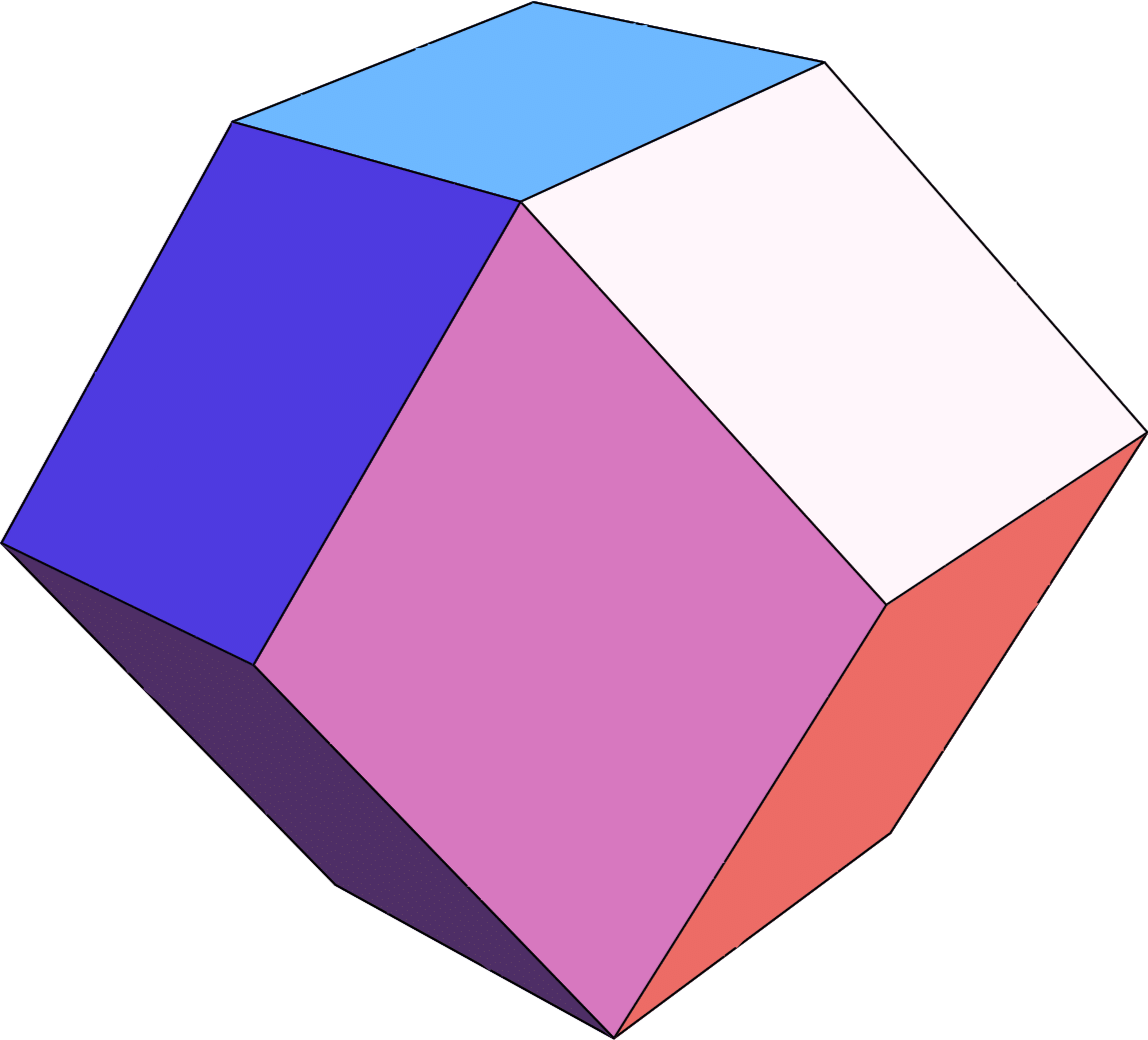
\includegraphics[height=6cm]{RhombicDodecahedron.png}
            
            \caption{A rhombic dodecahedron.}\label{fig:RhombicDodecahedron}
            
        \end{center}
        
    \end{figure}

    \begin{enumerate}
        \item The Voronoi cell has 12 faces (note these are codimension one faces, which are 2 dimensional).
        Of these we choose three pairwise intersecting ones, thus forming a cancellation-free basis: let $F_{C_1}$ be the top right (white) face of the dodecahedron, $F_{C_2}$ be the top (light blue) face, and $F_{C_3}$ be the front (light purple) face.
        \item There are 24 edges, which belong to four parallel classes (of 6 edges each).
        Let $\epsilon_1$ be the edge between the two left side faces (dark blue and dark purple), $\epsilon_2$ be the edge between the two right side faces (white and orange), $\epsilon_3$ be the edge between the front and top left faces (light purple and dark blue), and $\epsilon_4$ be the edge between the front and top right faces (light purple and white).
    
        Note that each face is a parallelogram, so they contain two pairs of parallel edges.
        The parallel classes $\{[\epsilon_2], [\epsilon_4]\}$ appear in $F_{C_1}$, $\{[\epsilon_1], [\epsilon_2]\}$ appear in $F_{C_2}$, and $\{[\epsilon_3], [\epsilon_4]\}$ appear in $F_{C_3}$.
        \item The equations are given as follows.
        Firstly, for the equations given by \eqref{eq:CircuitPairing}: for $C_1$, the parallel classes of edges $[\epsilon_1]$ and $[\epsilon_3]$ do not participate, so $n_1+n_3=\iprod*{C_1, C_1}=3$, similarly, for $C_2$ we have $n_3+n_4=3$ and for $C_3$ we have $n_1+n_2=4$.
        For the equations given by \eqref{eq:CircuitIntersection}: for $C_1, C_2$, the parallel class of edges $[\epsilon_3]$ does not participate, so $n_3=\iprod*{C_1, C_2}=1$, similarly, for $C_1, C_3$ we have $n_1=2$ and for $C_2, C_3$ we have $0=0$, as all parallel classes of edges participate in the faces corresponding to $C_2, C_3$.
        \item Solving this system of linear equations gives $n_1=2, n_2=2, n_3=1, n_4=2$.
        \item There are $7$ elements in the base set, let $S_1=\{e_1, e_2\}, S_2=\{e_3, e_4\}, S_3=\{e_5\}, S_4=\{e_6, e_7\}$ where $\abs*{S_i}=n_i$, then $E(\calM)=\cup_{i=1}^4 S_i=\{e_1, \dots, e_7\}$.
        \item There are six (unoriented) circuits corresponding to the $6$ pairs of parallel faces, that is each of the visible faces in \cref{fig:RhombicDodecahedron} and their corresponding parallel face on the opposite (non-visible) side.
        Then we have the three circuits we described, $C_1$ corresponding to the top right (white) face, $C_2$ corresponding to the top (light blue) face and $C_3$ corresponding to the front (light purple) face.
        We also have three more corresponding to the other faces, which are linear combinations of the circuit basis circuits above, namely $C_4=C_3+C_2-C_1$ corresponding to the top left (dark blue) face, $C_5=C_1-C_2$ corresponding to the bottom right (orange) face and $C_6=C_3-C_1$ corresponding to the bottom left (dark purple) face.
        Then the circuits are made up of the union of $S_i$ where the parallel class of edges $[\epsilon_i]$ does not participate in the face.
        So for $C_1$, as it contains the parallel classes of edges $\{[\epsilon_2], [\epsilon_4]\}$, the circuit is $C_1=S_1\cup S_3=\{e_1, e_2, e_5\}$.
        Similarly,
    
        \[\begin{aligned}
            C_2&=S_3\cup S_4=\{e_5, e_6, e_7\}\\
            C_3&=S_1\cup S_2=\{e_1, e_2, e_3, e_4\}\\
            C_4&=S_2\cup S_4=\{e_3, e_4, e_6, e_7\}\\
            C_5&=S_1\cup S_4=\{e_1, e_2, e_6, e_7\}\\
            C_6&=S_2\cup S_3=\{e_3, e_4, e_5\}.
        \end{aligned}\]
        So the matroid is $\calM$ with $E(\calM)=\{e_1, \dots, e_7\}$ and $\calC(\calM)=\{C_1, \dots, C_6\}$ as above.
    \end{enumerate}

\end{example}

In fact this is a graphical matroid, so we can find a representing graph by drawing out the cycles.
A representing graph is given in \cref{fig:ReconstructedGraph}, note that this is only a representing graph up to 2-isomorphism and up to extra non-participating vertices.

\begin{figure}[htbp]

    \begin{center}
    
        \begin{tikzpicture}
        
            \node[shape=circle, draw=black, fill=black] (A) at (0,0) {};
            \node[shape=circle, draw=black, fill=black] (B) at (-2,2) {};
            \node[shape=circle, draw=black, fill=black] (C) at (0,4) {};
            \node[shape=circle, draw=black, fill=black] (D) at (2,2) {};
            \node[shape=circle, draw=black, fill=black] (E) at (4,2) {};
        
            \draw (C) -- (D) node[midway, left] {$e_1$};
            \draw (A) -- (D) node[midway, left] {$e_2$};
            \draw (A) -- (B) node[midway, left] {$e_3$};
            \draw (B) -- (C) node[midway, left] {$e_4$};
            \draw (A) -- (C) node[midway, right] {$e_5$};
            \draw (A) -- (E) node[midway, right] {$e_6$};
            \draw (C) -- (E) node[midway, right] {$e_7$};
    
        \end{tikzpicture}
    
    \end{center}

    \caption{A graph $G$ representing the 2-isomorphism class for the graphical matroid $\calM$ reconstructed in \cref{ex:Reconstruction}.}\label{fig:ReconstructedGraph}

\end{figure}

\begin{figure}[htbp]

    \begin{center}
    
        \begin{tikzpicture}
        
            \node[shape=circle, draw=black, fill=black, label=below:$v_1$] (A) at (0,0) {};
            \node[shape=circle, draw=black, fill=black, label=left:$v_2$] (B) at (-2,2) {};
            \node[shape=circle, draw=black, fill=black, label=above:$v_3$] (C) at (0,4) {};
            \node[shape=circle, draw=black, fill=black, label=right:$v_4$] (D) at (2,2) {};
            \node[shape=circle, draw=black, fill=black, label=right:$v_5$] (E) at (4,2) {};
        
            \draw[->-] (D) -- (C) node[midway, below left] {$e_1$};
            \draw[->-] (A) -- (D) node[midway, above left] {$e_2$};
            \draw[->-] (B) -- (A) node[midway, below left] {$e_3$};
            \draw[->-] (C) -- (B) node[midway, above left] {$e_4$};
            \draw[->-] (C) -- (A) node[midway, right] {$e_5$};
            \draw[->-] (A) -- (E) node[midway, below right] {$e_6$};
            \draw[->-] (E) -- (C) node[midway, above right] {$e_7$};
    
        \end{tikzpicture}
    
    \end{center}

    \caption{A graph $G$ representing the 2-isomorphism class of the matroid $\calM$ reconstructed in \cref{ex:Reconstruction}, with an orientation applied.}\label{fig:OrientedReconstructedGraph}

\end{figure}

Applying the orientation given in \cref{fig:OrientedReconstructedGraph}, and arbitrarily labelling the vertices, we can write the signed incidence matrix.

\[\begin{bmatrix}
    0 & -1 & 1 & 0 & 1 & -1 & 0\\
    0 & 0 & -1 & 1 & 0 & 0 & 0\\
    1 & 0 & 0 & -1 & -1 & 0 & 1\\
    -1 & 1 & 0 & 0 & 0 & 0 & 0\\
    0 & 0 & 0 & 0 & 0 & 1 & -1
\end{bmatrix}\]

Indeed, with the choice of circuit basis  $C_1=\{+e_1, +e_2, +e_5\}, C_2=\{+e_5, +e_6, +e_7\}, C_3=\{+e_1, +e_2, +e_3, +e_4\}$, we obtain

\[\begin{aligned}
    \iprod*{C_1, C_1}&=3\\
    \iprod*{C_2, C_2}&=3\\
    \iprod*{C_3, C_3}&=4\\
    \iprod*{C_1, C_2}&=1\\
    \iprod*{C_1, C_3}&=2\\
    \iprod*{C_2, C_3}&=0,
\end{aligned}\]
and this results in the same Gram matrix as the one we started out with:

\[\begin{pmatrix}
    3 & 1 & 2\\
    1 & 3 & 0\\
    2 & 0 & 4
\end{pmatrix}.\]

\newpage

\printbibliography[title=References]

\end{document}